\section{Systemarchitektur}\label{sec:systemarchitektur}

Es gibt 3 große Services, das Chat Widget auf der Schulhomepage, das Dashboard und das Backend.
Unser System sieht folgendermaßen aus:

\begin{figure}[hbt!]
    \centering
    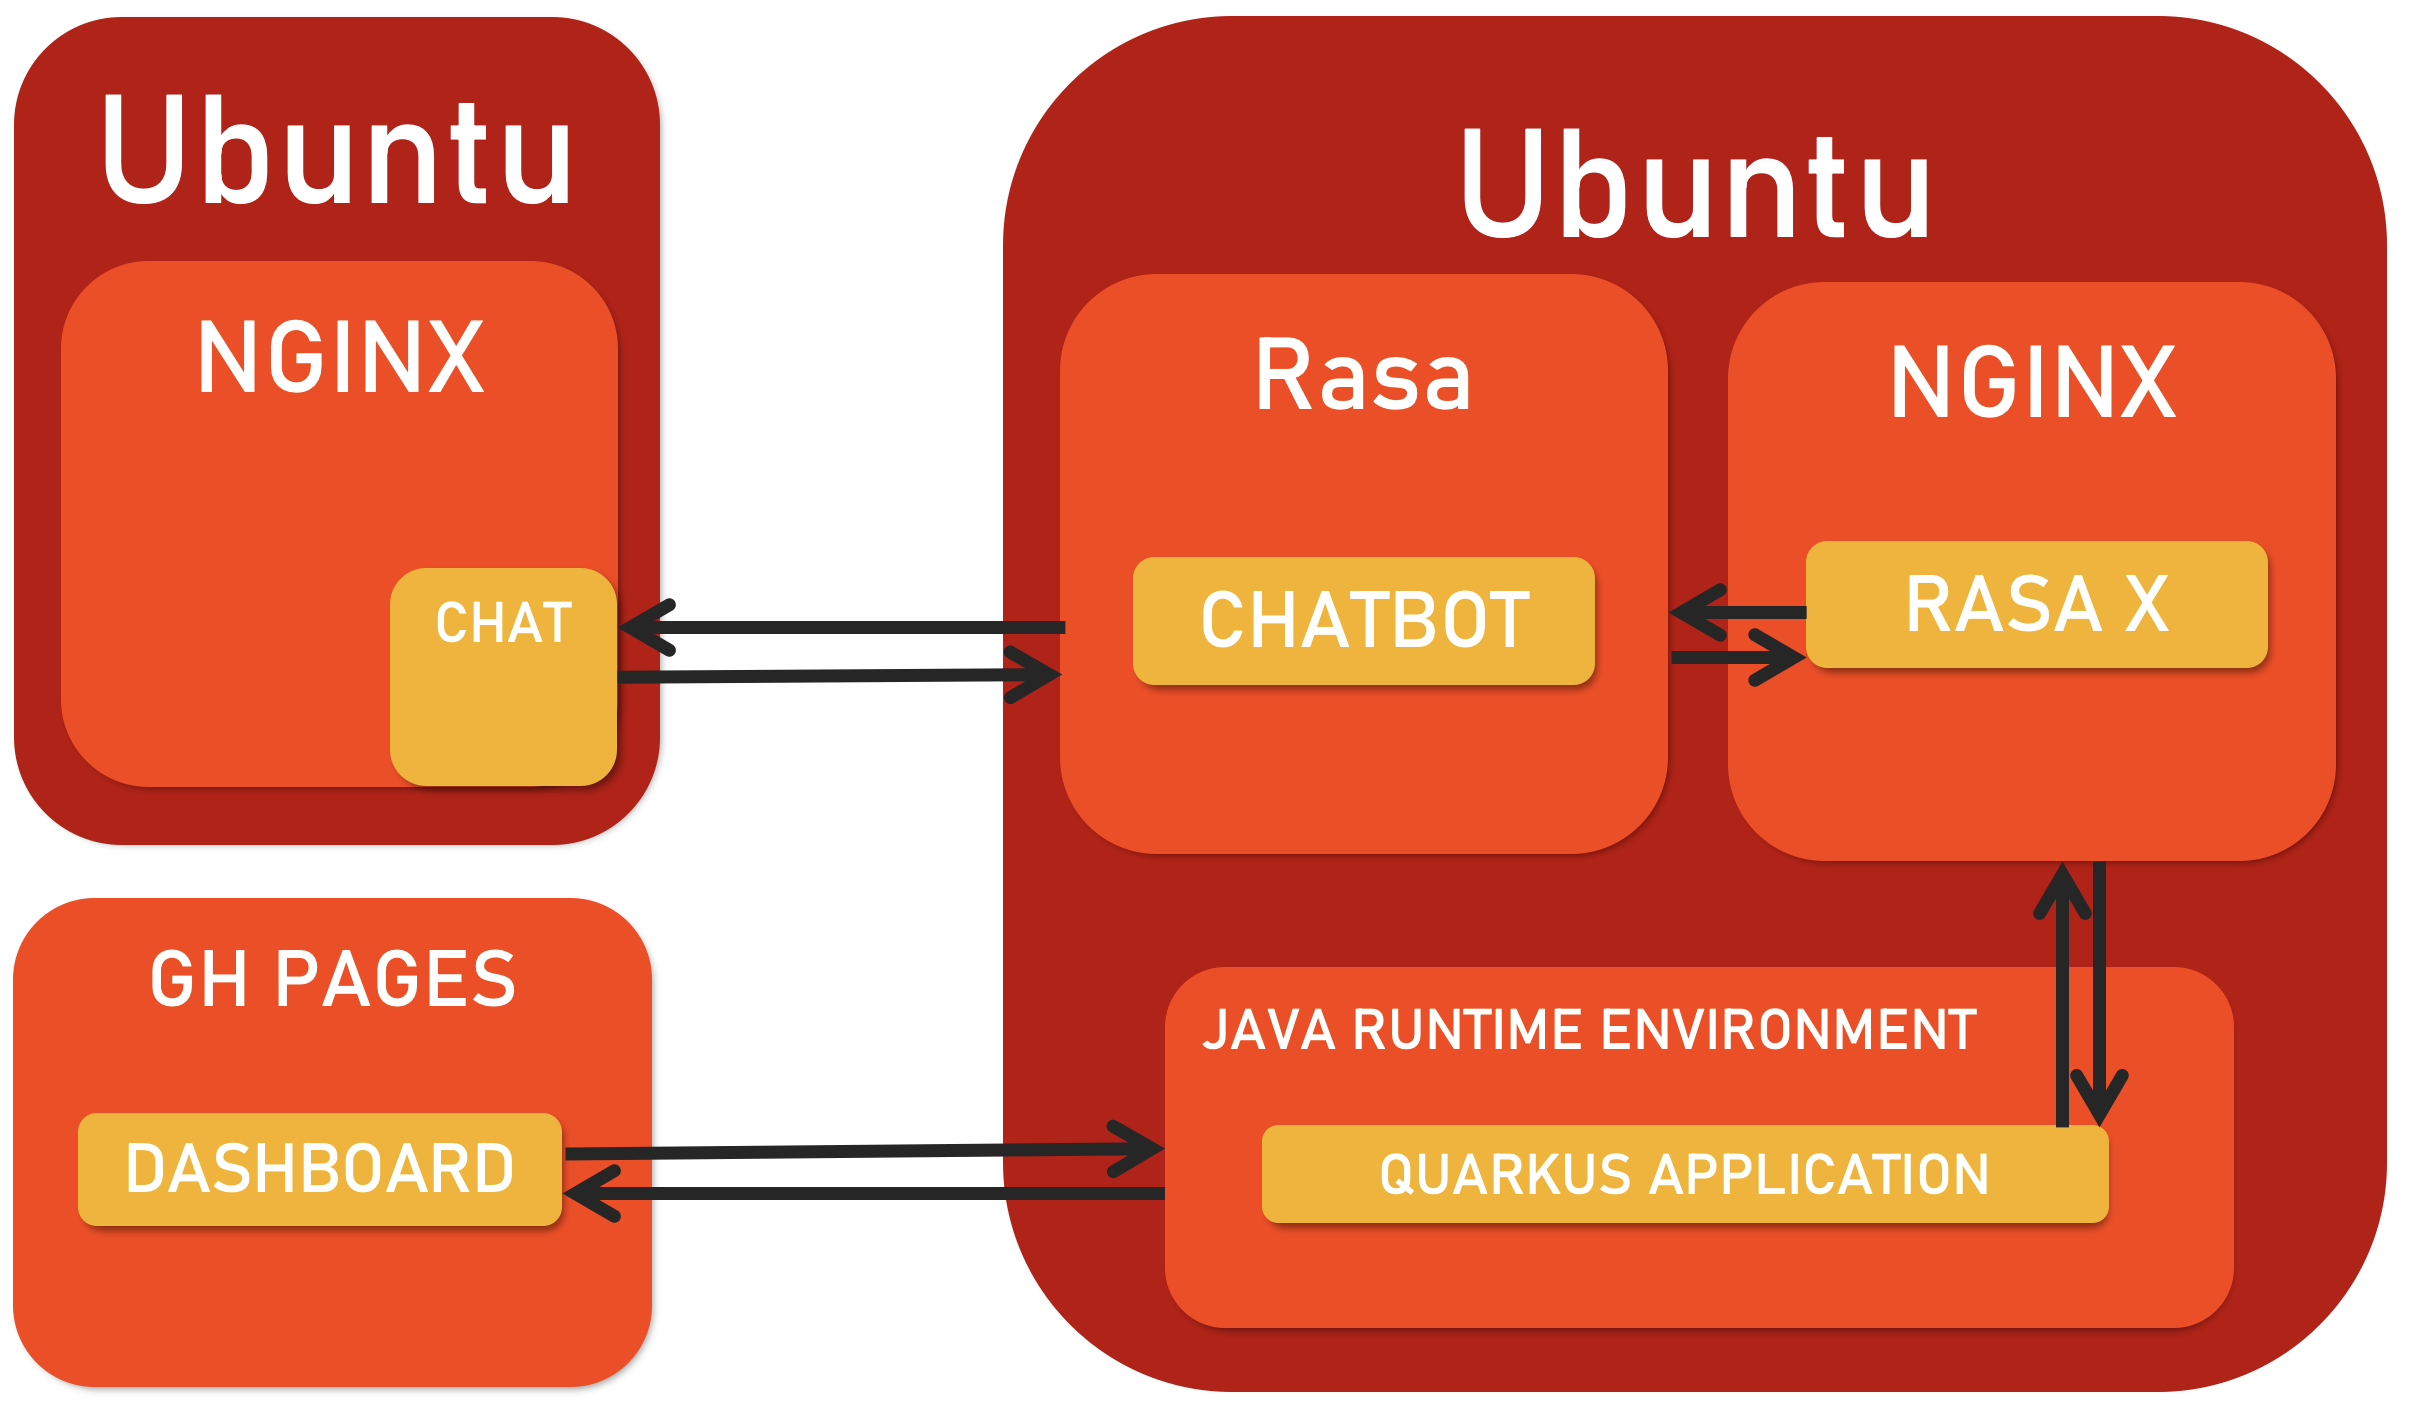
\includegraphics[scale=0.2]{pics/systemarchitektur}
    \caption{Systemarchitektur}
    \label{fig:impl:architektur}
\end{figure}

Es gibt 2 Ubuntu VM's, eine für den Chat und eine für Rasa und das Backend, nachdem der Chat auf die HTL Leonding Seite kommt, wird dadurch nur noch eine VM benötigt.

Unser Chat wird gerade mit NGINX gehostet, dieser kommuniziert mit Rasa direkt über REST, wenn der Benutzer eine Nachricht sendet, wird diese an Rasa gesendet und Rasa antwortet mit der passenden Antwort.
Das Dashboard wird auf GH Pages gehostet, dieses kommuniziert mit dem Backend über REST, das Backend authentisiert sich bei Rasa X ~\ref{subsec:rasa-x} und holt sich alle Konversationen und bereitet diese auf und sendet sie an das Dashboard.

\section{Backend}\label{sec:backend}
\setauthor{Felix Dumfarth}

Unser Quarkus ~\ref{quarkus} Backend hat die Aufgabe mit Rasa X zu kommunizieren und die Konversationsdaten für das Dashboard aufzubereiten und zu senden.

Unser Backend besitzt folgende Endpoints:

\begin{itemize}
    \item GET /api/conversations
    \item GET /api/conversations/{id}
    \item POST /api/feedback
    \item GET /api/feedback
    \item GET /api/file/{filename}
    \item PUT /api/file/{filename}
\end{itemize}

Bei den beiden ``conversations'' endpoints muss man sich aber zuerst authentisieren und sich einen Bearer Token von Rasa x holen damit man auf die anderen Rasa X endpoints zugreifen kann.

\subsection{GET /api/conversations}
Der Endpoint ruft zuerst die getAuth() funktion auf, um den Bearer Token zu erhalten.

Danach wird der Rasa X GET Endpoint ``/api/conversations'' aufgerufen, mit dem Bearer Token im Header.
Von diesem Endpoint wird ein JSON Objekt zurückgegeben, das die Konversationen enthält, aber zusätzlich noch viele andere unrelevante Daten, deshalb filtert sich das Backend wirklich nur ID des Senders, die Zeit und die Anzahl von Nachrichten der Unterhaltungen heraus und gibt diese zurück.

\subsection{GET /api/conversations/{id}}
Der Endpoint /api/conversations/{id} ruft zuerst die getAuth() funktion auf, um den Bearer Token zu erhalten.

Um nur von einer gezielten Unterhaltung die Nachrichten zu erhalten wird der Rasa X Endpoint ``/api/conversations/{id}/messages'' aufgerufen, mit dem Bearer Token im Header.
Die Response wird auch in dieser Form schon zurückgeben, da die Response keine unwichtigen Daten enthält.

\subsection{POST /api/feedback}
Der Endpoint /api/feedback erhält ein JSON Objekt mit den Daten des Feedback Formulars und speichert diese in die Datenbank.

\subsection{GET /api/feedback}
Der Endpoint /api/feedback liest alle Feedbacks aus der Datenbank aus und gibt diese zurück.

\subsection{GET /api/file/{filename}}
Der Endpoint /api/file/{filename} liest die im URL angegeben Datei aus dem Filesystem aus und gibt diese zurück.
Die möglichen Dateinamen sind:

\begin{itemize}
    \item nlu.yml
    \item rules.yml
    \item stories.yml
    \item config.yml
    \item domain.yml
\end{itemize}

\subsection{PUT /api/file/{filename}}
Der Endpoint /api/file/{filename} erhält den Inhalt aus dem File welches auch im URL angegeben wurde und überschreibt dieses dann im Filesystem.

\section{Chat Widget}\label{sec:chat-widget}
Der Chatbot der HTL Leonding sollte auf der Schulhomepage als Chatblase angezeigt werden, und verschiedene Elemente wie Buttons und Links unterstützen.

\subsection{Konzept}
Während den Anfängen der vorliegenden Arbeit wurde ein Konzept erstellt, um das mögliche Aussehen festzulegen.
Lange Zeit wurde der Chatbot, während der Entwicklung, unter den Namen Leon geführt.
Dies wurde jedoch im späteren Verlauf geändert und Leon wurde Teil des langjährigen Leonie Projektes der HTL Leonding.

\begin{figure}[hbt!]
    \centering
    \includegraphics[scale=0.2]{pics/conceptBotClosed}
    \caption{Konzept Chatbot geschlossen}
    \label{fig:impl:conceptBotClosed}
\end{figure}
\begin{figure}[hbt!]
    \centering
    \includegraphics[scale=0.2]{pics/conceptBotOpen}
    \caption{Konzept Chatbot geöffnet}
    \label{fig:impl:conceptBotOpen}
\end{figure}

\subsection{Umsetzung}
Umgesetzt wurde das Frontend mithilfe von Angular.
Die Chatblase ist eine eigene Komponente, die durch CSS immer rechts unten fixiert ist.
Die Farben des Chatbots sollten natürlich an die HTL Leonding erinnern, deshalb wurde ein Farbverlauf aus Farben des HTL Logos erstellt.

Jedoch begann der Chatbot sehr anders, zu begin wurde der Bot zuerst als ganze Seite entwickelt und nicht nur als Chatblase.
\begin{figure}[hbt!]
    \centering
    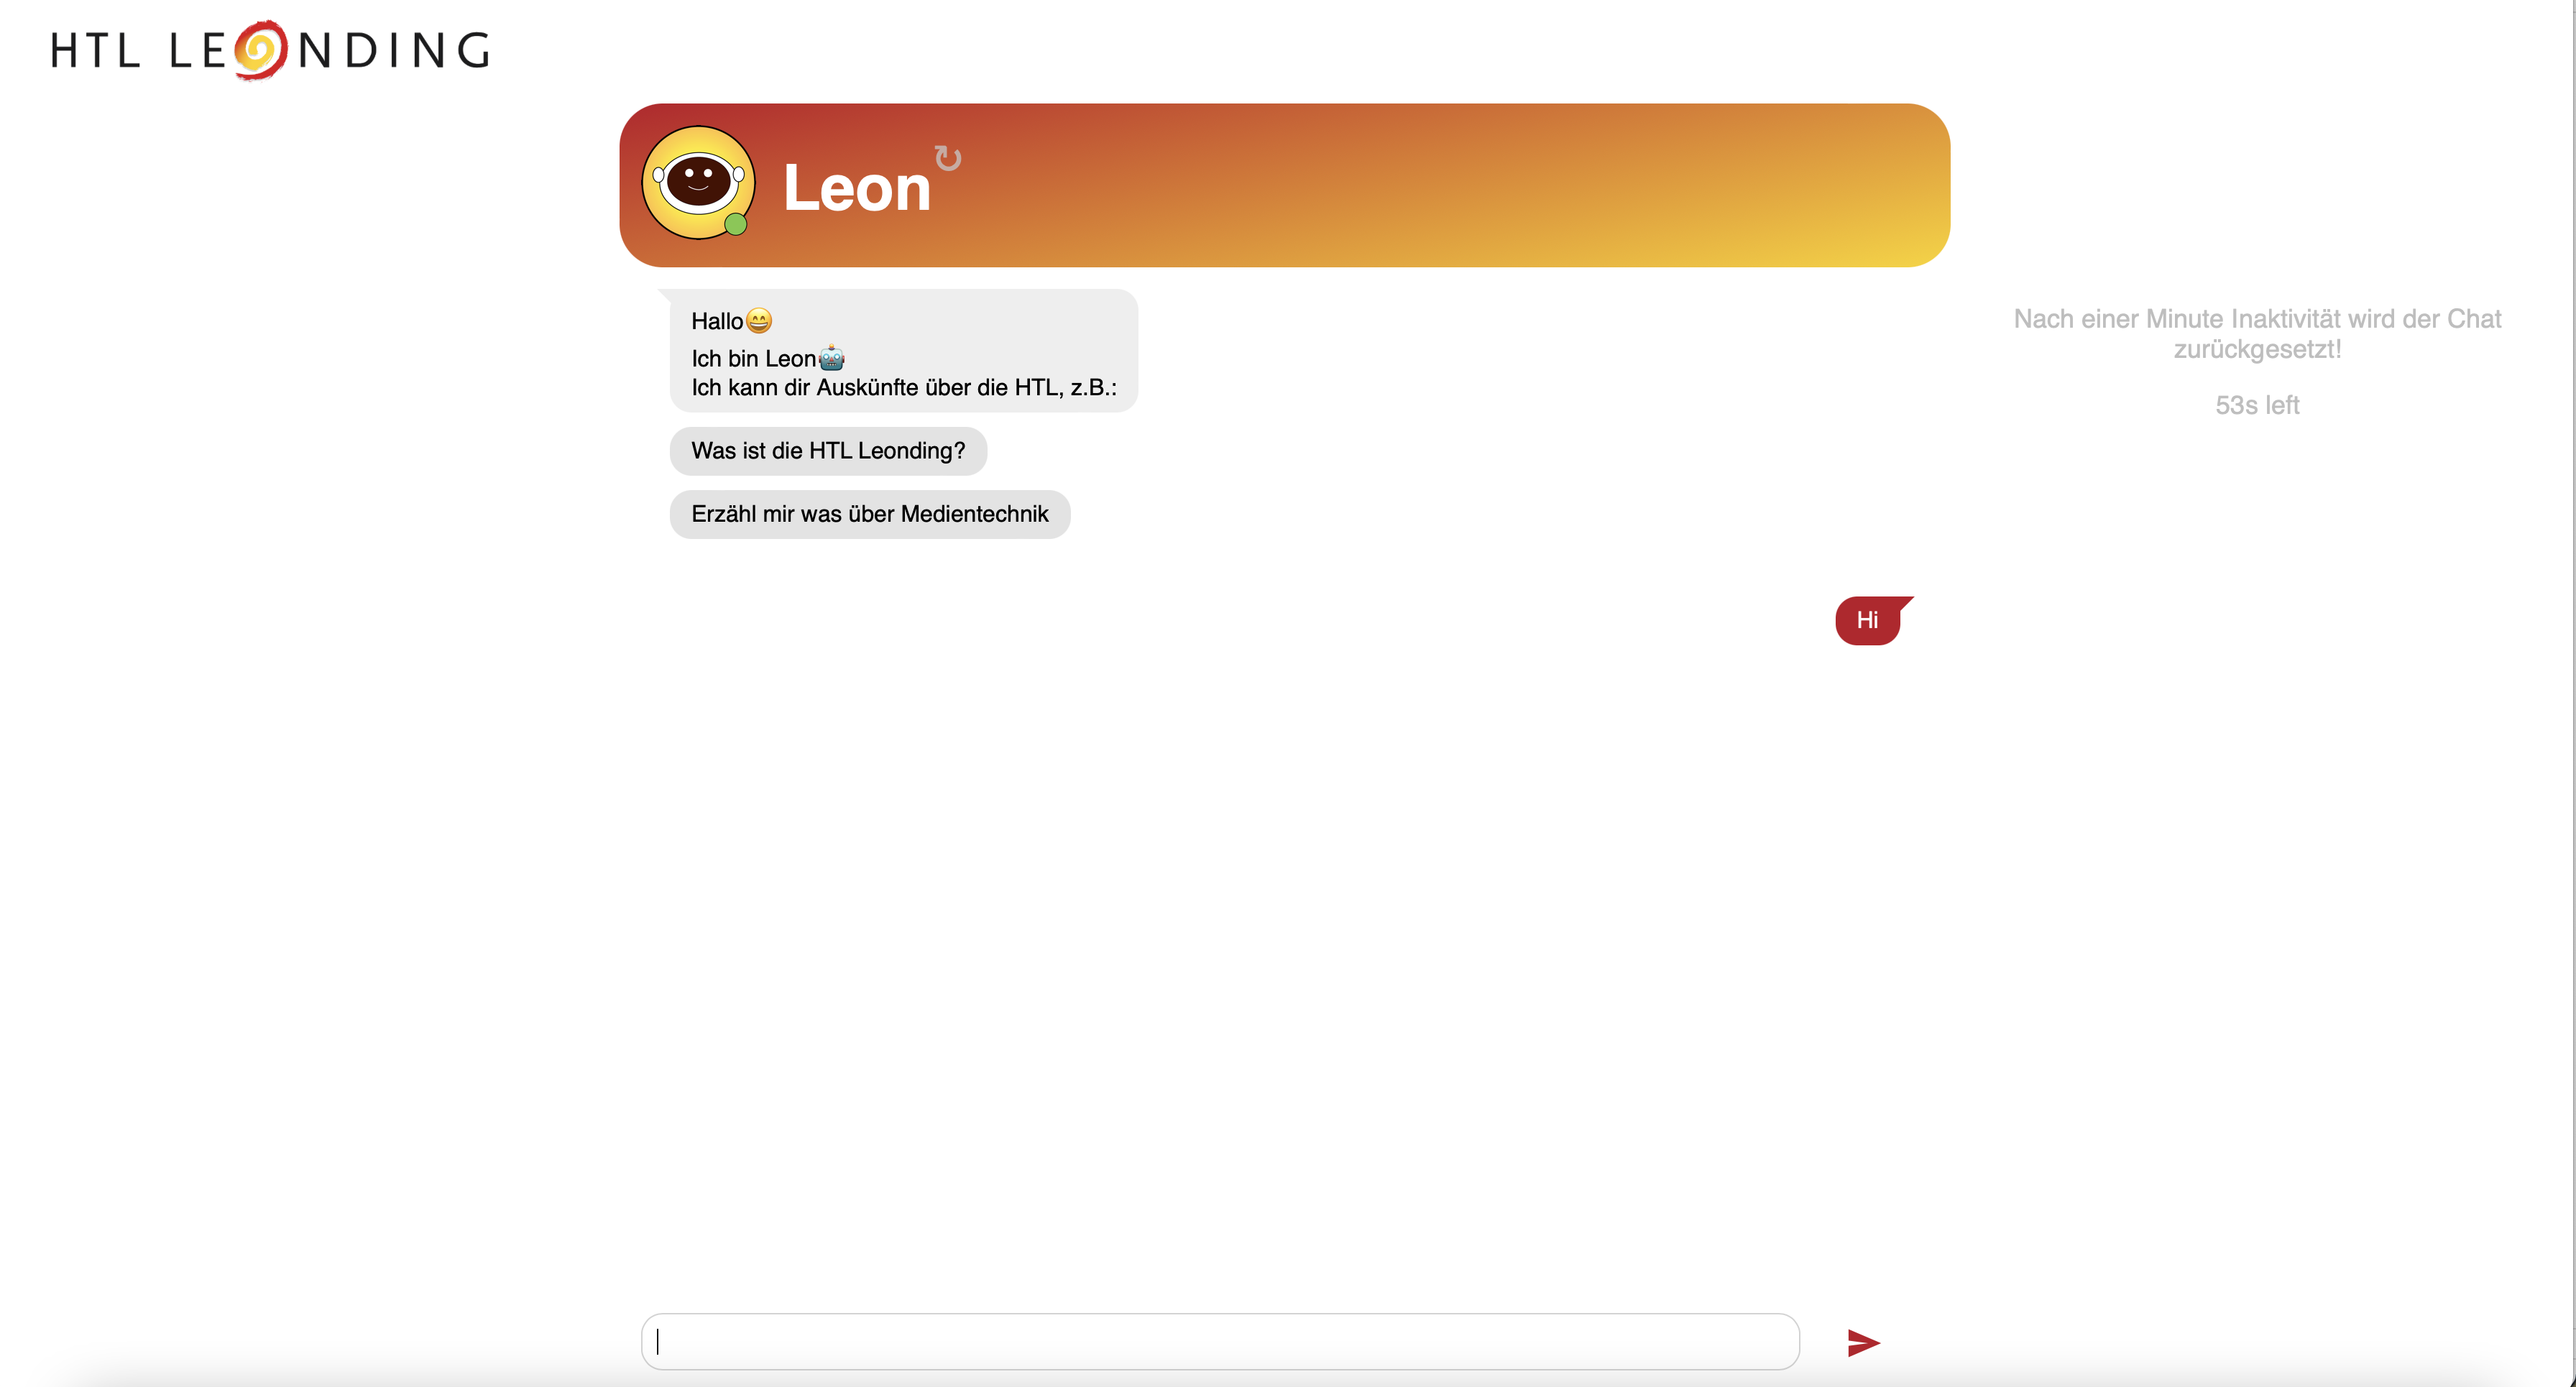
\includegraphics[scale=0.2]{pics/fullPageBot}
    \caption{Chatbot auf einer ganzen Seite}
    \label{fig:impl:conceptBotFullPage}
\end{figure}

Natürlich war dies nicht das endgültige Ziel so wurde der Bot schnell zur Chatblase umgewandelt.
Zum Testen war die HTL Leonding Seite mithilfe eines IFrames eingebunden und zusätzlich die Chatblasen Komponente.

Um das Gespräch in eine Richtung zu lenken wurden Buttons eingeführt, die nach fast jeder Antwort mögliche folge Fragen vorschlagen.

\begin{figure}[hbt!]
    \centering
    \includegraphics[scale=0.2]{pics/finalBot.png}
    \caption{Chatbot}
    \label{fig:impl:bot}
\end{figure}

Die Buttons werden von Rasa mit der Antwort auf die Frage mitgeschickt, wenn ein Benutzter auf einen der Buttons drückt wird nicht der Text des Buttons an Rasa geschickt sondern direkt die Bezeichnung des Intents mit einem ``/'' davor, da Rasa dies auch erkennt.

Um Bewertungen von echten Benutzern zu holen wurde außerdem eine Feedback Seite eingeführt, in dieser kann der Benutzer eine 1 bis 5 Sterne bewertung und einen Text absenden.

\begin{figure}[hbt!]
    \centering
    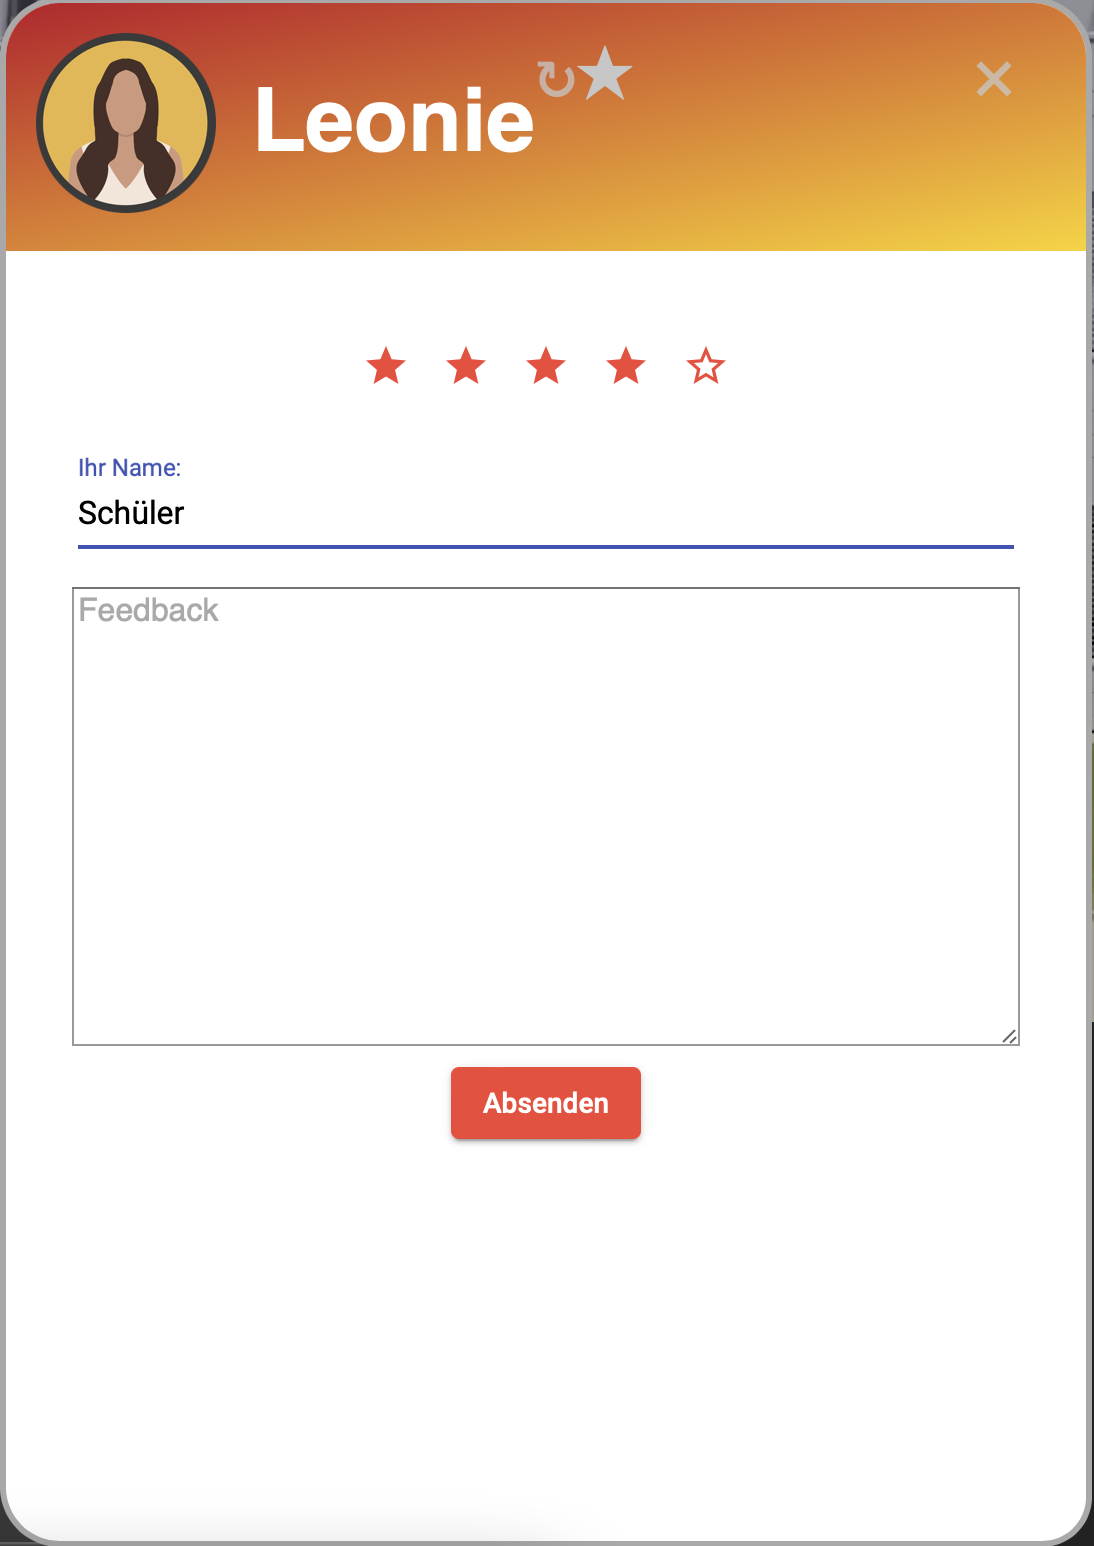
\includegraphics[scale=0.3]{pics/feedback}
    \caption{Feedback Fenster}
    \label{fig:impl:feedback}
\end{figure}

Das Chatfenster wurde in wesentliche 3 Bereiche geteilt.

\begin{figure}[hbt!]
    \centering
    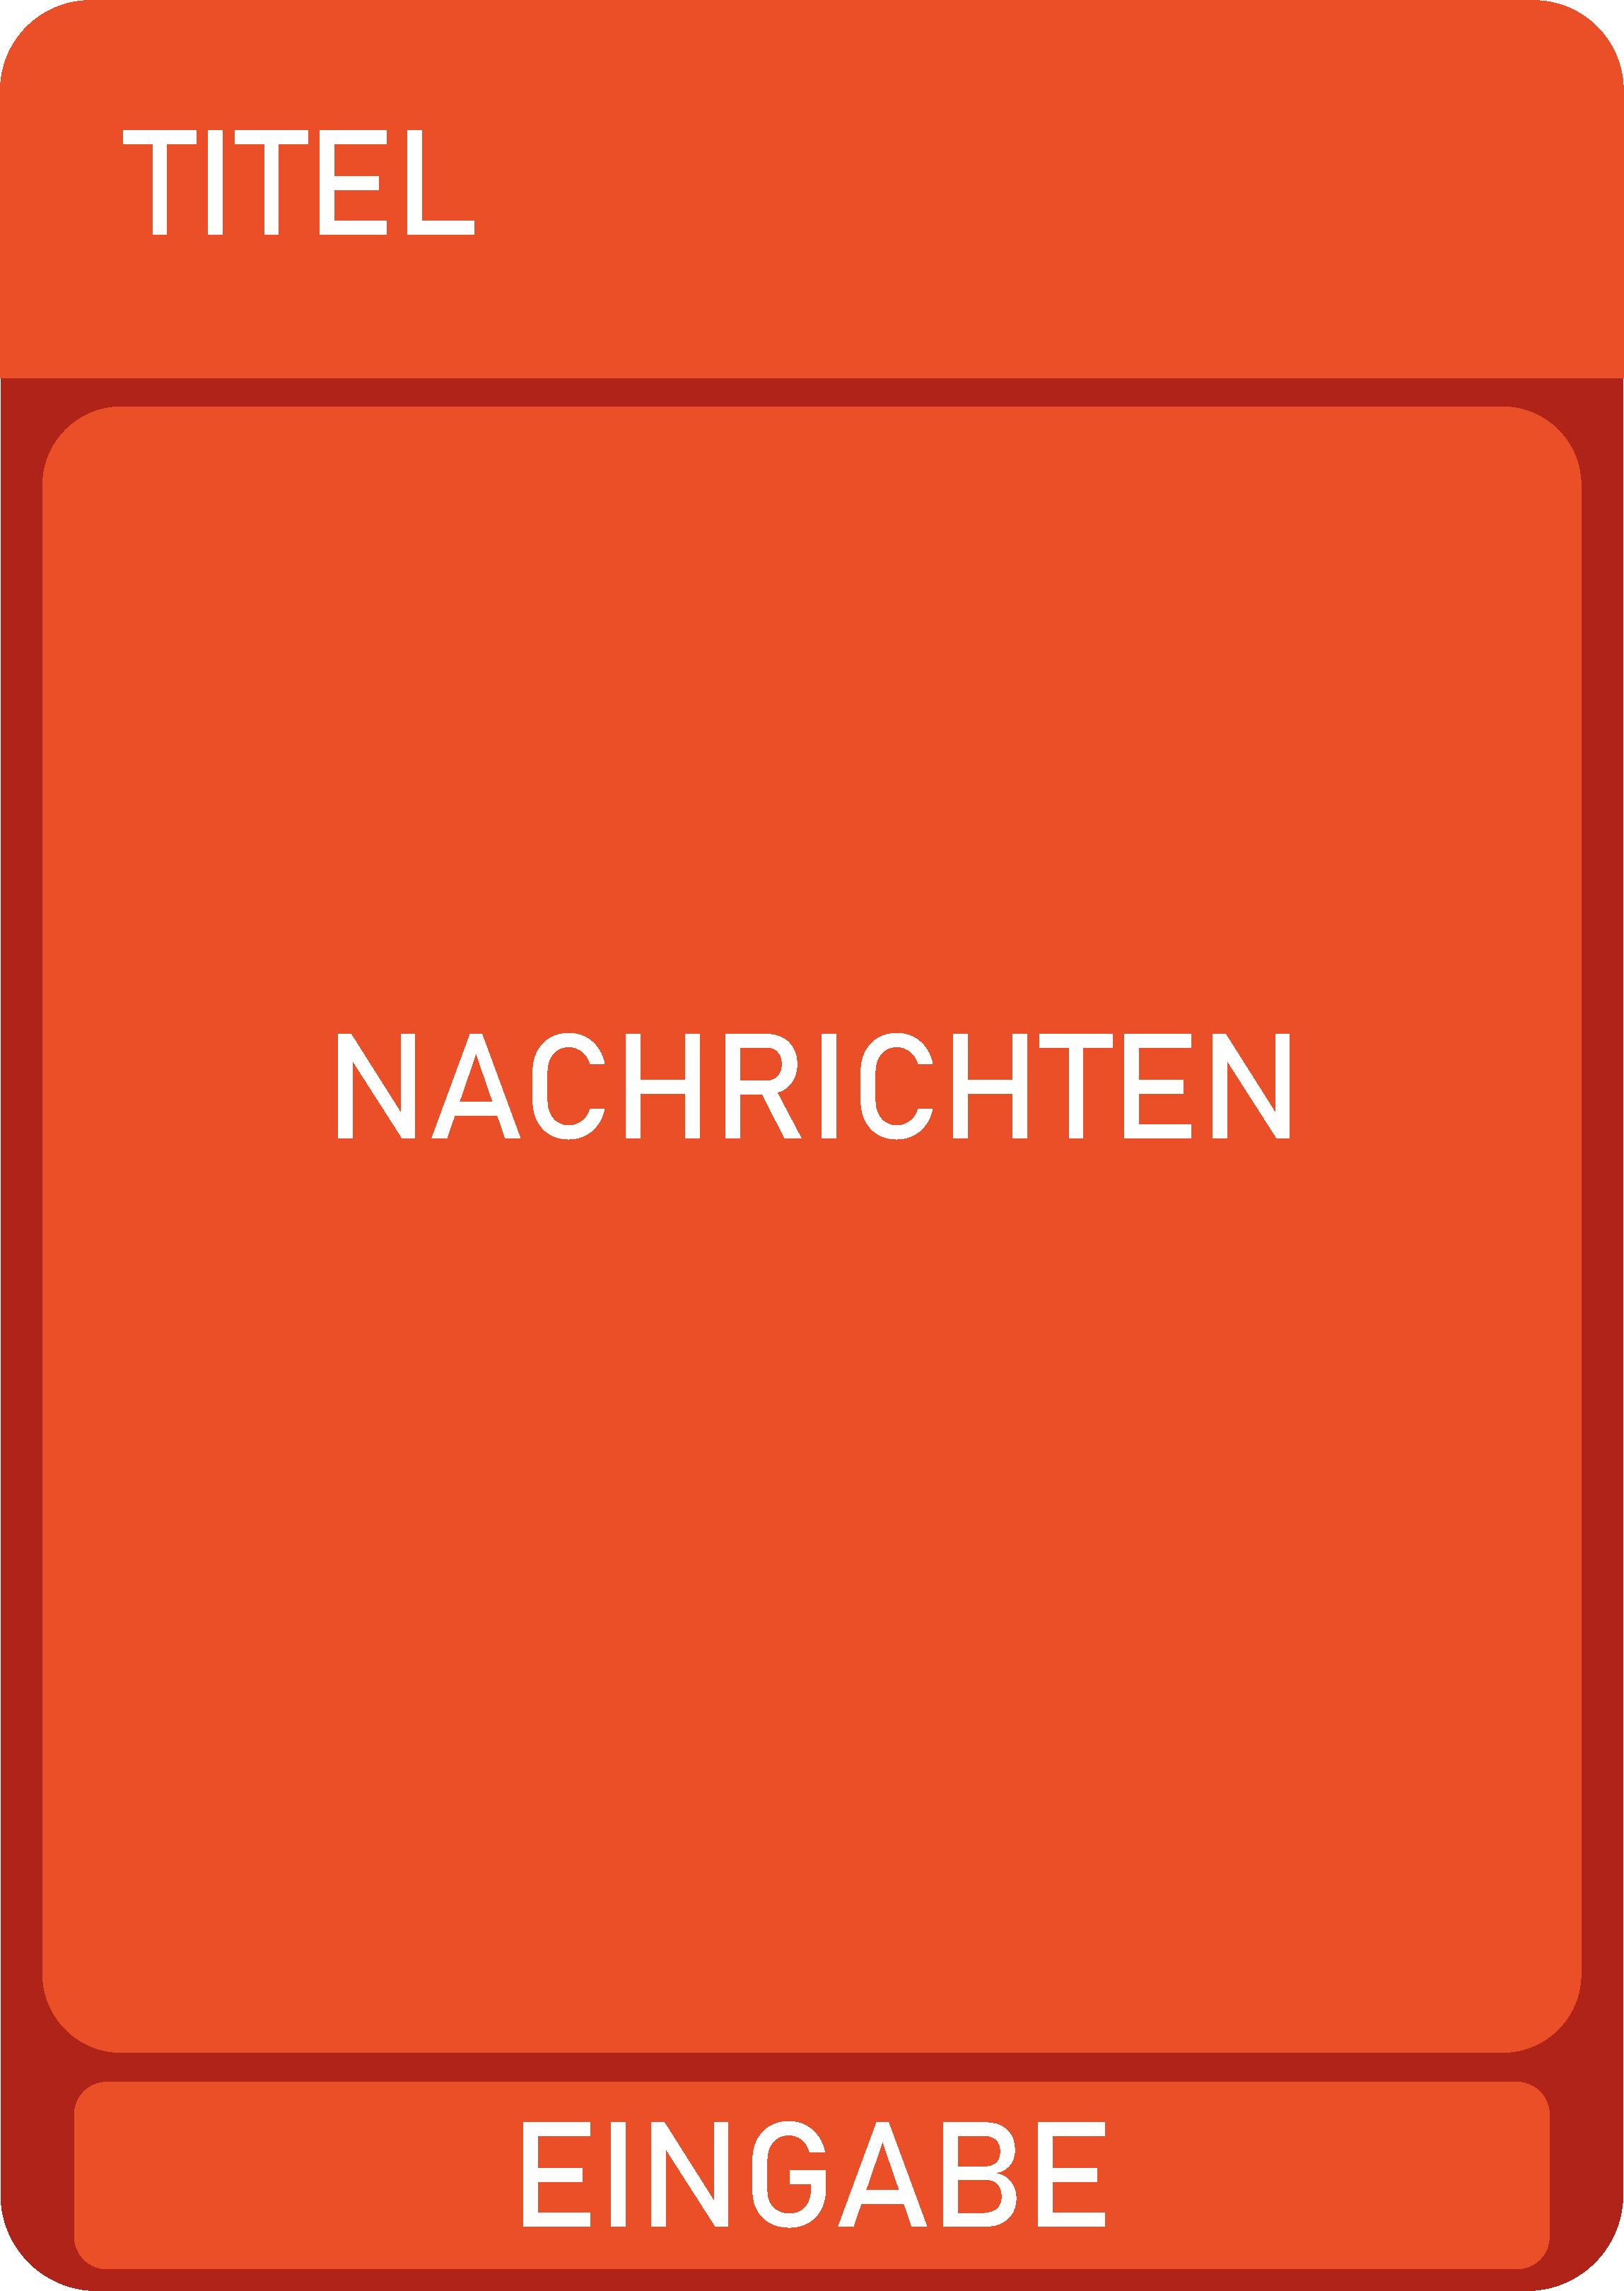
\includegraphics[scale=0.4]{pics/chatWidgetStructure}
    \caption{Aufbau vom Chat Fenster}
    \label{fig:impl:chatWidget}
\end{figure}

\subsubsection{Avatar}
Wie bereits erwähnt existiert der Virtuelle Avatar der Leonie bereits in Form einer 3D Pyramide und einer Webseite mit einem 3D Modell, das Interessierte Person nicht mit zu vielen virtuellen ``Personen'' verwirrt werden wurde entschieden das unser Chatbot auch als ``Leonie'' bekannt sein soll.
Die alte Leonie war ein 3D Model, dies würde aber nicht ganz zu einem Profilbild im Chat passen.
\begin{figure}[hbt!]
    \centering
    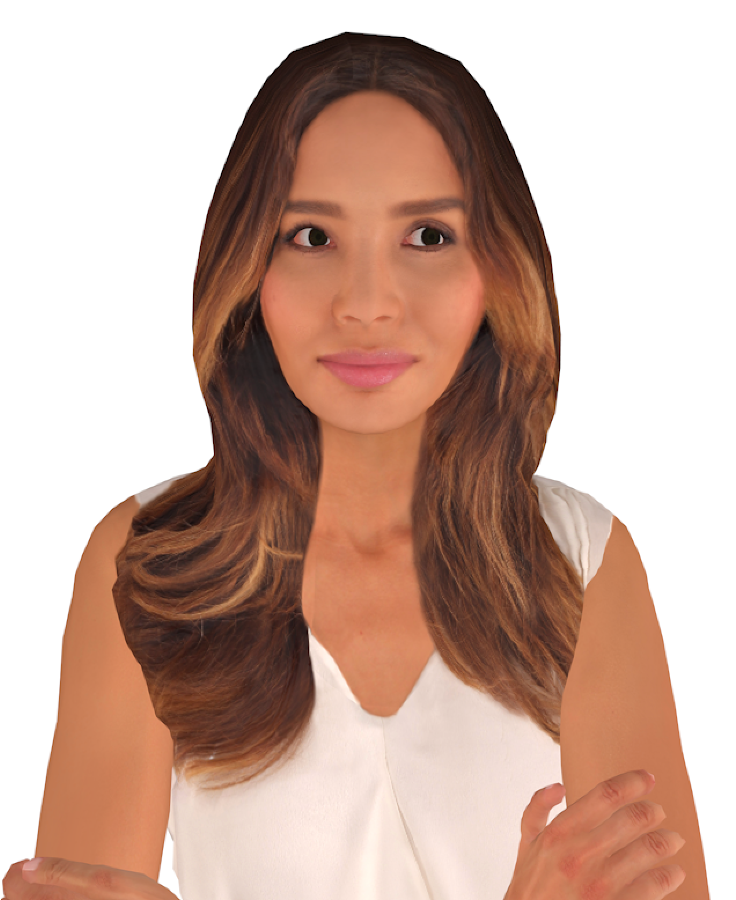
\includegraphics[scale=0.5]{pics/AvatarLeonie}
    \caption{3D Leonie}
    \label{fig:impl:leonie}
\end{figure}

Es würde mit ``Adobe Illustrator'' eine 2D Grafik erstellt, die eine färbige Silhouette der 3D Leonie darstellt.

\begin{figure}[hbt!]
    \centering
    
\includegraphics[scale=0.3]{pics/LeonieTrans}
    \caption{2D Leonie}
    \label{fig:impl:leonieTrans}
\end{figure}

\section{Dashboard}\label{sec:dashboard}

Um alle Gespräche und die Bewertungen der Benutzer anzuzeigen wurde ein Dashboard eingeführt, wo nur dies möglich war.
Im Laufe der Arbeit wurde dieses dann erweitert, um für den Leobot Conversation Cycle als Seite zu dienen.

\subsection{Conversation-Driven Development}\label{cdd}
Rasa empfiehlt für die Entwicklung von Chatbots ``Conversation-Driven Development'', kurz CDD.\cite{cdd}
Aber was ist CDD?

CDD beschreibt eine Entwicklungsstrategie, in der du deinen Chatbot nach Konversationen mit echten Usern verbesserst.

Bei CDD wird empfohlen, dass man seinen Chatbot möglichst früh echten Benutzern zur verfügung stehlt und so beobachten kann was die echten Benutzer alles für Intents erwarten und wie sie ihre Anfragen formulieren und kann diese bei Bedarf hinzufügen.



\subsection{Leobot Conversation Cycle}

\begin{figure}[hbt!]
    \centering
    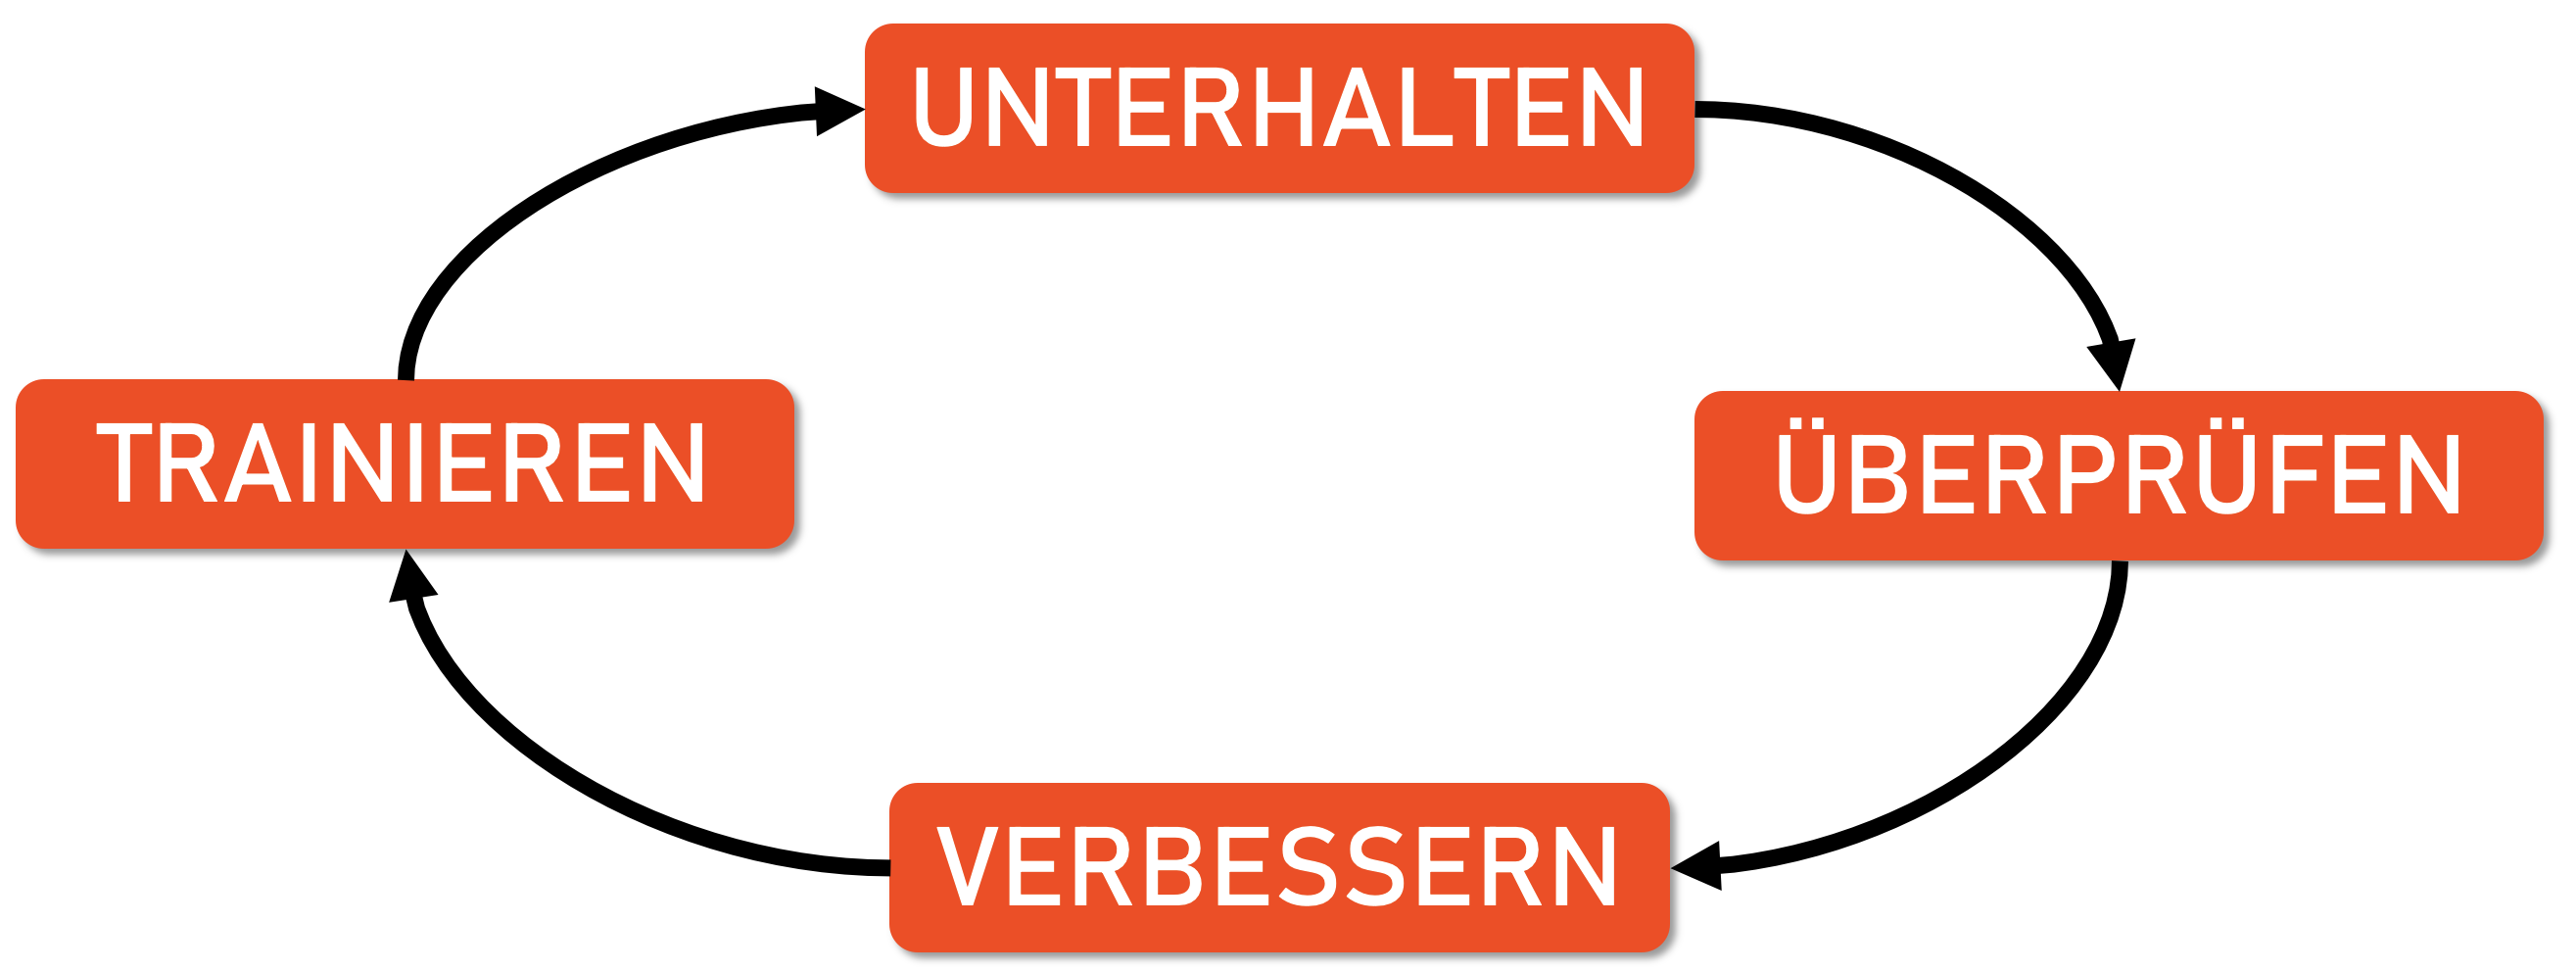
\includegraphics[scale=0.2]{pics/LeoCircle}
    \caption{Leobot Conversation Cycle}
    \label{fig:impl:ConversationCycle}
\end{figure}

CDD ~\ref{cdd} wird mithilfe unsres Leobot Conversation Cycle um, der Leobot Conversation Cycle ist ein Workflow, der dazu dient, den Leobot zu überprüfen und zu erweitern.

Der Workflow besteht aus folgenden Schritten:

\begin{itemize}
    \item Unterhalten
    \item Überprüfen
    \item Verbessern
    \item Trainieren
\end{itemize}

Diese 4 Schritte werden immer wieder durchgeführt, um den Chatbot dauerhaft zu verbessern.

\subsubsection{Unterhalten}
Unterhalten ist der erste Schritt des Leobot Conversation Cycles, in diesem Schritt werden dem Bot Fragen über die HTL Leonding und deren Produktangebot gestellt, die er beantworten muss, dies passiert während Unterhaltungen im Chat auf der Schulhomepage mit echten Personen.
Diese Unterhaltungen werden dann alle gespeichert.

\subsubsection{Überprüfen}

Überprüfen ist der zweite Schritt des Leobot Conversation Cycles, in diesem Schritt wird der Bot vom Schulpersonal oder Verantwortlichen überprüft, ob dieser die Fragen richtig beantwortet und erkannt hat oder ob Verbesserungspotential besteht

\subsubsection{Verbessern}
Verbessern ist der dritte Schritt des Leobot Conversation Cycles, in diesem Schritt wird der Bot verbessert, das heißt die Fehler werden versucht zu beheben.
Je nachdem was der fehler des Bots war muss hier anders gearbeitet werden.
Wenn er einen Intent den er eigentlich kennt aber die Formulierung des Benutzers so war das er diesen nicht erkannt hat, wird die Eingabe des Benutzers zu den Trainingsdaten hinzugefügt.

Falls jemand aber eine Frage stellt zu der es keinen Intent gibt und sich die Verantwortlichen denken es wäre ein guter Intent so wird der ganze Intent zu den Trainingsdaten hinzugefügt.

\subsubsection{Trainieren}
Trainieren ist der vierte Schritt des Leobot Conversation Cycles, in diesem Schritt werden die Trainingsdaten an den Bot übergeben und dieser Trainiert, nachdem er fertig trainiert wurde, wechselt auf das neu trainierte Model.

Und nun beginnt der Leobot Conversation Cycle wieder von vorne.

\subsubsection{Regelkreis}
\setauthor{Lukas Starka}

Dieser Vorgang erinnert dabei stark an einen Regelkreis.
Ein solcher Regelkreis ist in Abbildung ~\ref{fig:regelkreis} zu sehen und dieser führt eine Regelgröße auf einen gewünschten Sollwert.
Die Hauptkomponenten des Regelkreises sind der Regler und die Regelstrecke.
Beispielhaft ist die Regelstrecke ein Auto und die Fahrerin oder der Fahrer der Regler.
Dabei nimmt die Lenkerin oder der Lenker gewisse Parameter zur Hilfe, durch die entschieden wird, ob das Auto gelenkt, gebremst oder beschleunigt werden soll.
Diese Signale sind beispielsweise die aktuelle Geschwindigkeit, die Position des Autos oder die Fahrbahnverhältnisse.
Beim Regelkreis wird also eine Regelgröße über ein Eingangssignal der Regelstrecke zurückgeführt und auf einen gewünschten Wert gebracht.
Der Regelkreis wird oft bei der Regelung von Heizungen eingesetzt ~\ref{fig:heizungRegelKreis}.\cite{regelkreis, regelkreisBeispiel}

\begin{figure}[hbt!]
    \centering
    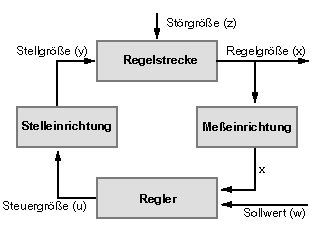
\includegraphics[scale=0.8]{pics/regelkreis}
    \caption{Allgemeiner Regelkreis ~\cite{regelkreis}}
    \label{fig:regelkreis}
\end{figure}

\begin{figure}[hbt!]
    \centering
    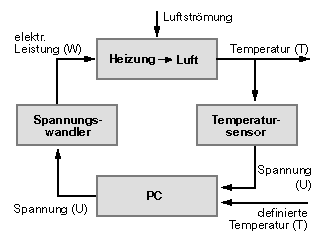
\includegraphics[scale=0.8]{pics/regelkreis_heizung}
    \caption{Regelkreis am Beispiel einer Heizung ~\cite{regelkreis}}
    \label{fig:heizungRegelKreis}
\end{figure}

Ein Regelkreis wird dabei entweder durch eine Änderung der Sollgröße oder durch Auftreten einer Störung ausgelöst.
Beim Leobot Conversation Cycle wird der Regelkreis demzufolge ausgelöst, wenn eine Interaktion mit einem User statt fand, bei der der Bot eine falsche Antwort gegeben hat.
Die Messeinrichtung ist dabei das Dashboard ~\ref{sec:dashboard}, das alle Unterhaltungen auflistet und diese grafisch veranschaulicht.
Durch den eingebauten Editor ist die Möglichkeit gegeben, dass direkt die Files bearbeitet werden, sodass der Bot in Zukunft auch auf diese Fragestellung die richtige Antwort parat hat.
Der Sollwert wird also in den Regler eingegeben und anschließend wird das Modell basierend auf den neuen Files neu trainiert.
Dies stellt dabei die Stelleinrichtung des Regelkreises dar und der Kreislauf kann von vorne beginnen, sollte erneut eine Störgröße auftreten oder die Sollgröße verändert werden.


\subsection{Warum das Dashboard}
\setauthor{Felix Dumfarth}
Rasa X bietet sehr viele Möglichkeiten auf einen Platz aber zu viele für Verwaltungspersonal das nicht unbedingt aus Programmierern besteht.
Die Oberfläche von Rasa X bietet Möglichkeiten Sachen zu verändern die man als normale Verwaltungsperson nicht unbedingt benötigt wie zum Beispiel Zugriff auf die Pipeline, Git und die ganzen trainierten Modele.
Das sind alles Funktionen die man als Verwaltungsperson nicht benötigt, man sollte wirklich nur das sehen was man auch verändern muss.

\subsection{Umsetzung}

\subsubsection{Authentifizierung}
Da nicht jeder auf das ``Gehirn'' des Bots zugreifen soll ist das Dashboard Benutzer und Passwort geschützt.
Außerdem soll in der Zukunft die Möglichkeit offen sein das manche Userrollen nur auf gewisse Inhalte zugriff haben.

Die Authentifizierung wird über das Backend mit property file based authentication\cite{authentication} durchgeführt.

\begin{figure}[hbt!]
    \centering
    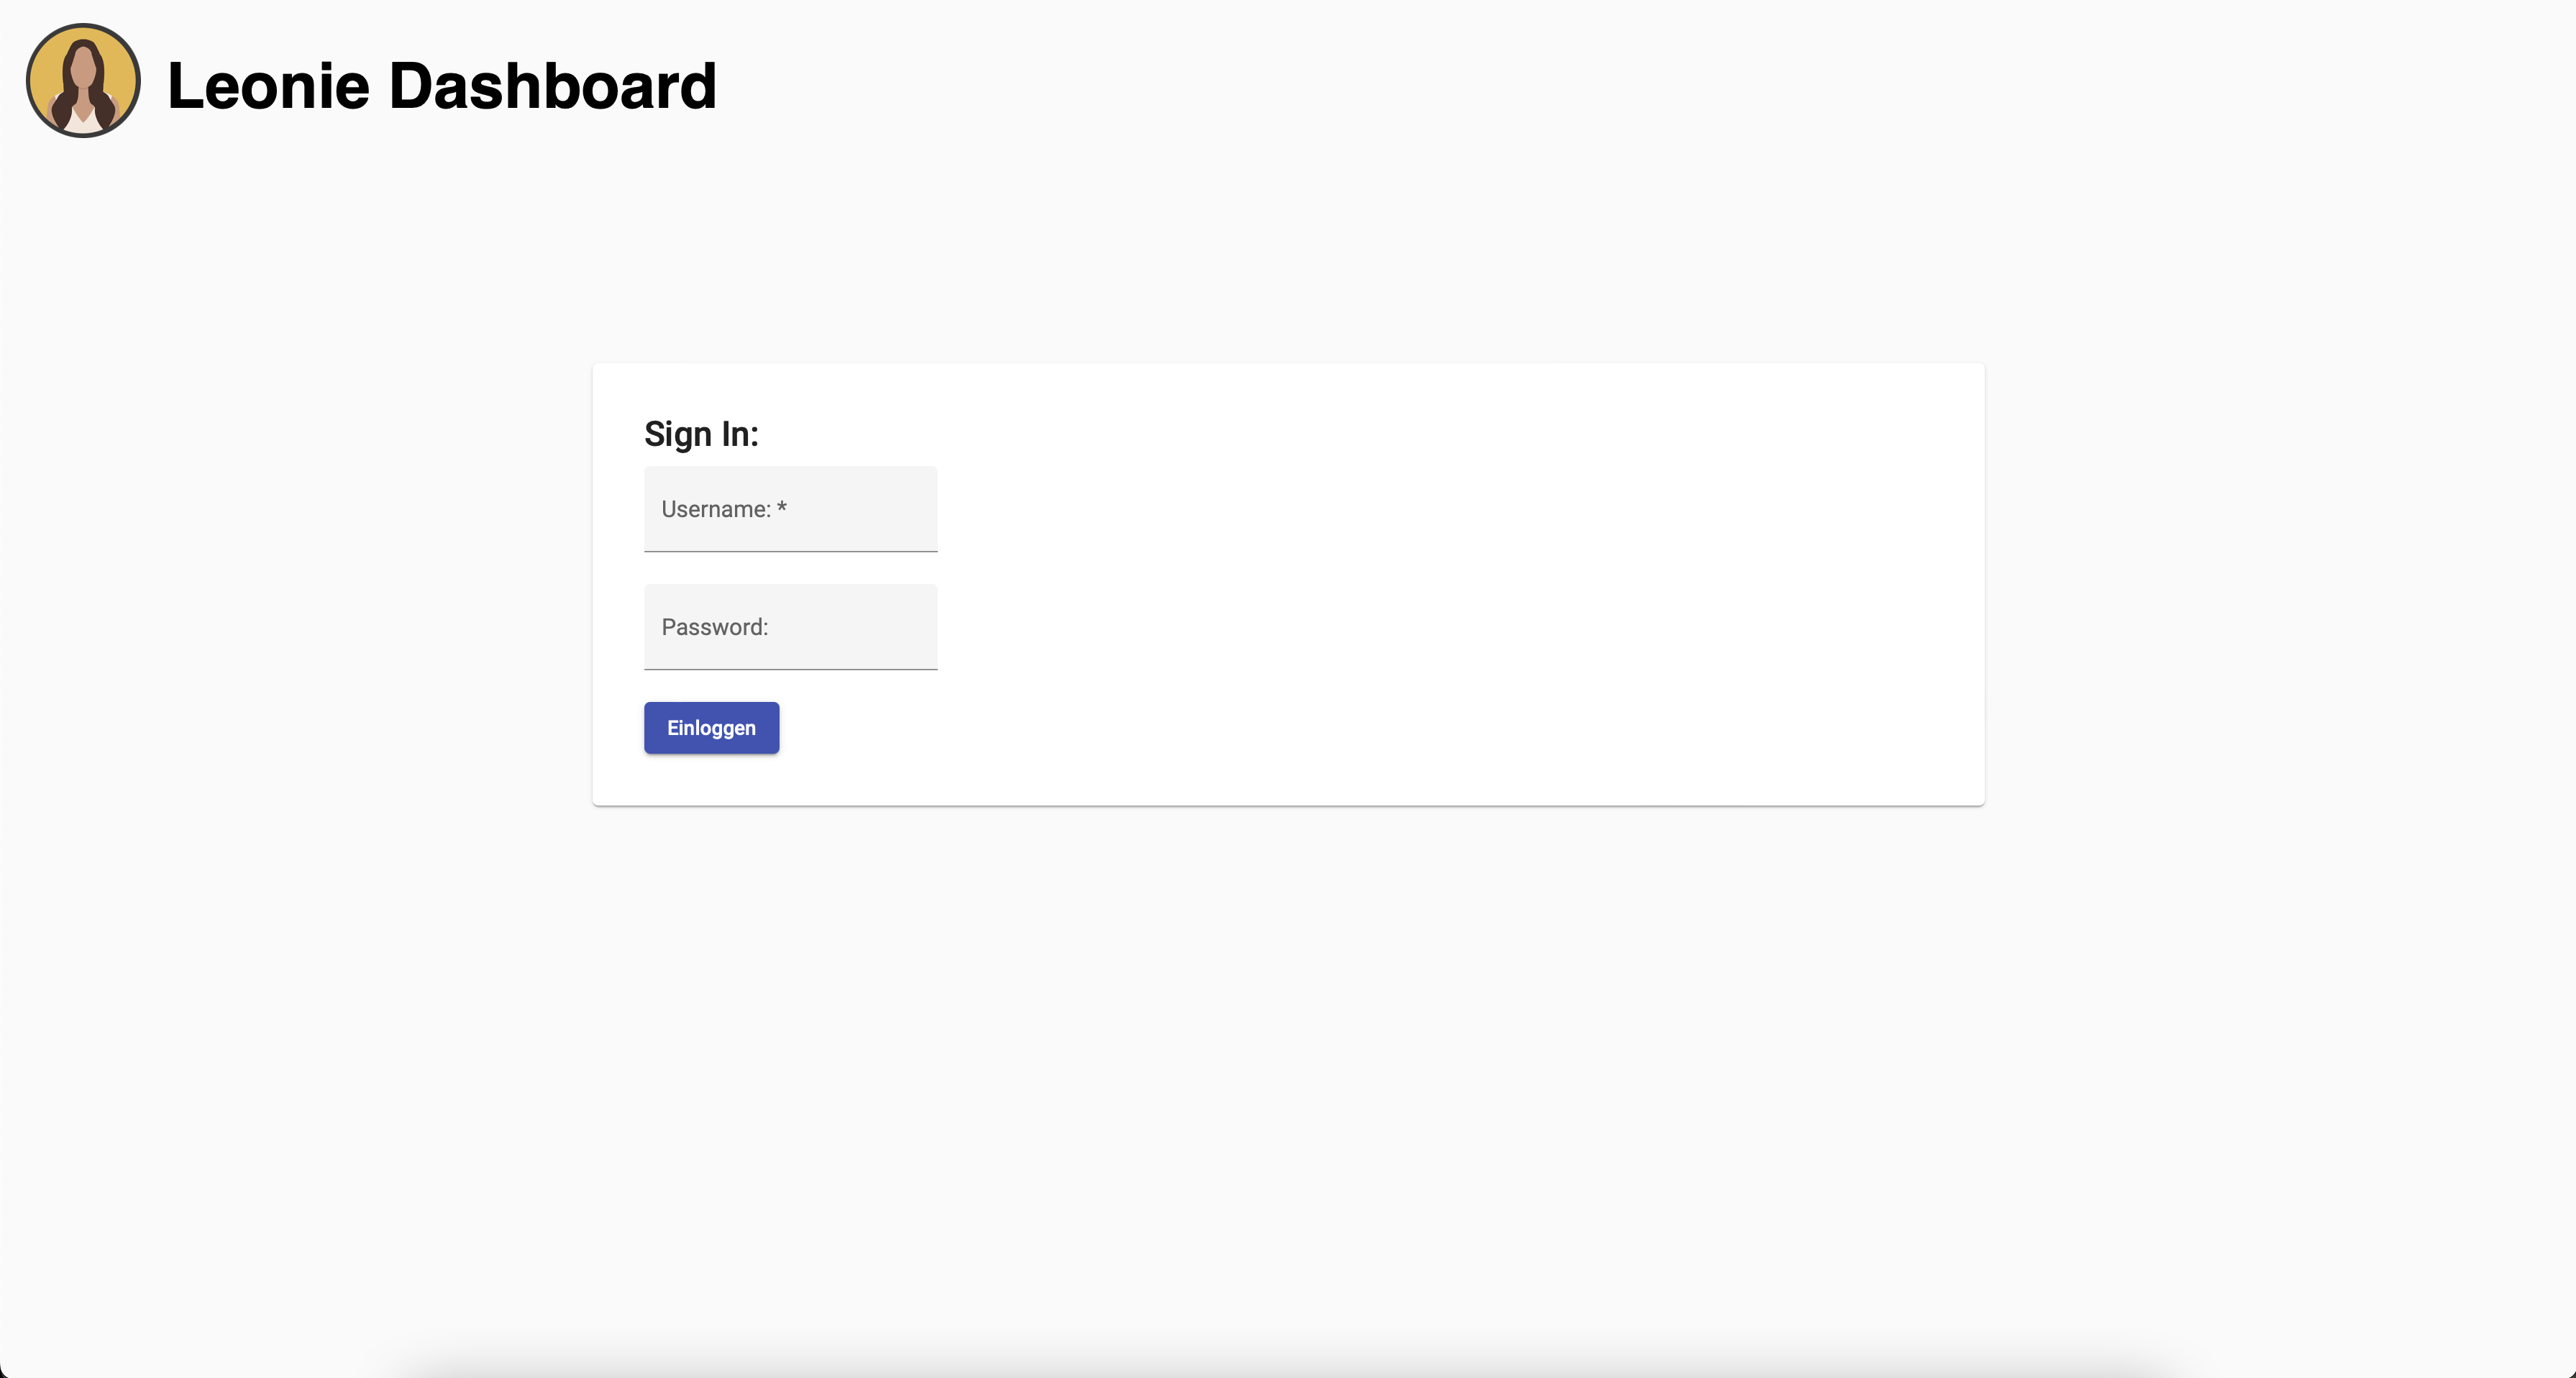
\includegraphics[scale=0.2]{pics/signin}
    \caption{Anmeldefenster}
    \label{fig:impl:signin}
\end{figure}

Einerseits kann man sich alle vergangenen Unterhaltungen ansehen, so wie die nlu.yml, stories.yml, rules.yml, domain.yml direkt im Monaco Editor bearbeiten und speichern.

\begin{figure}[hbt!]
    \centering
    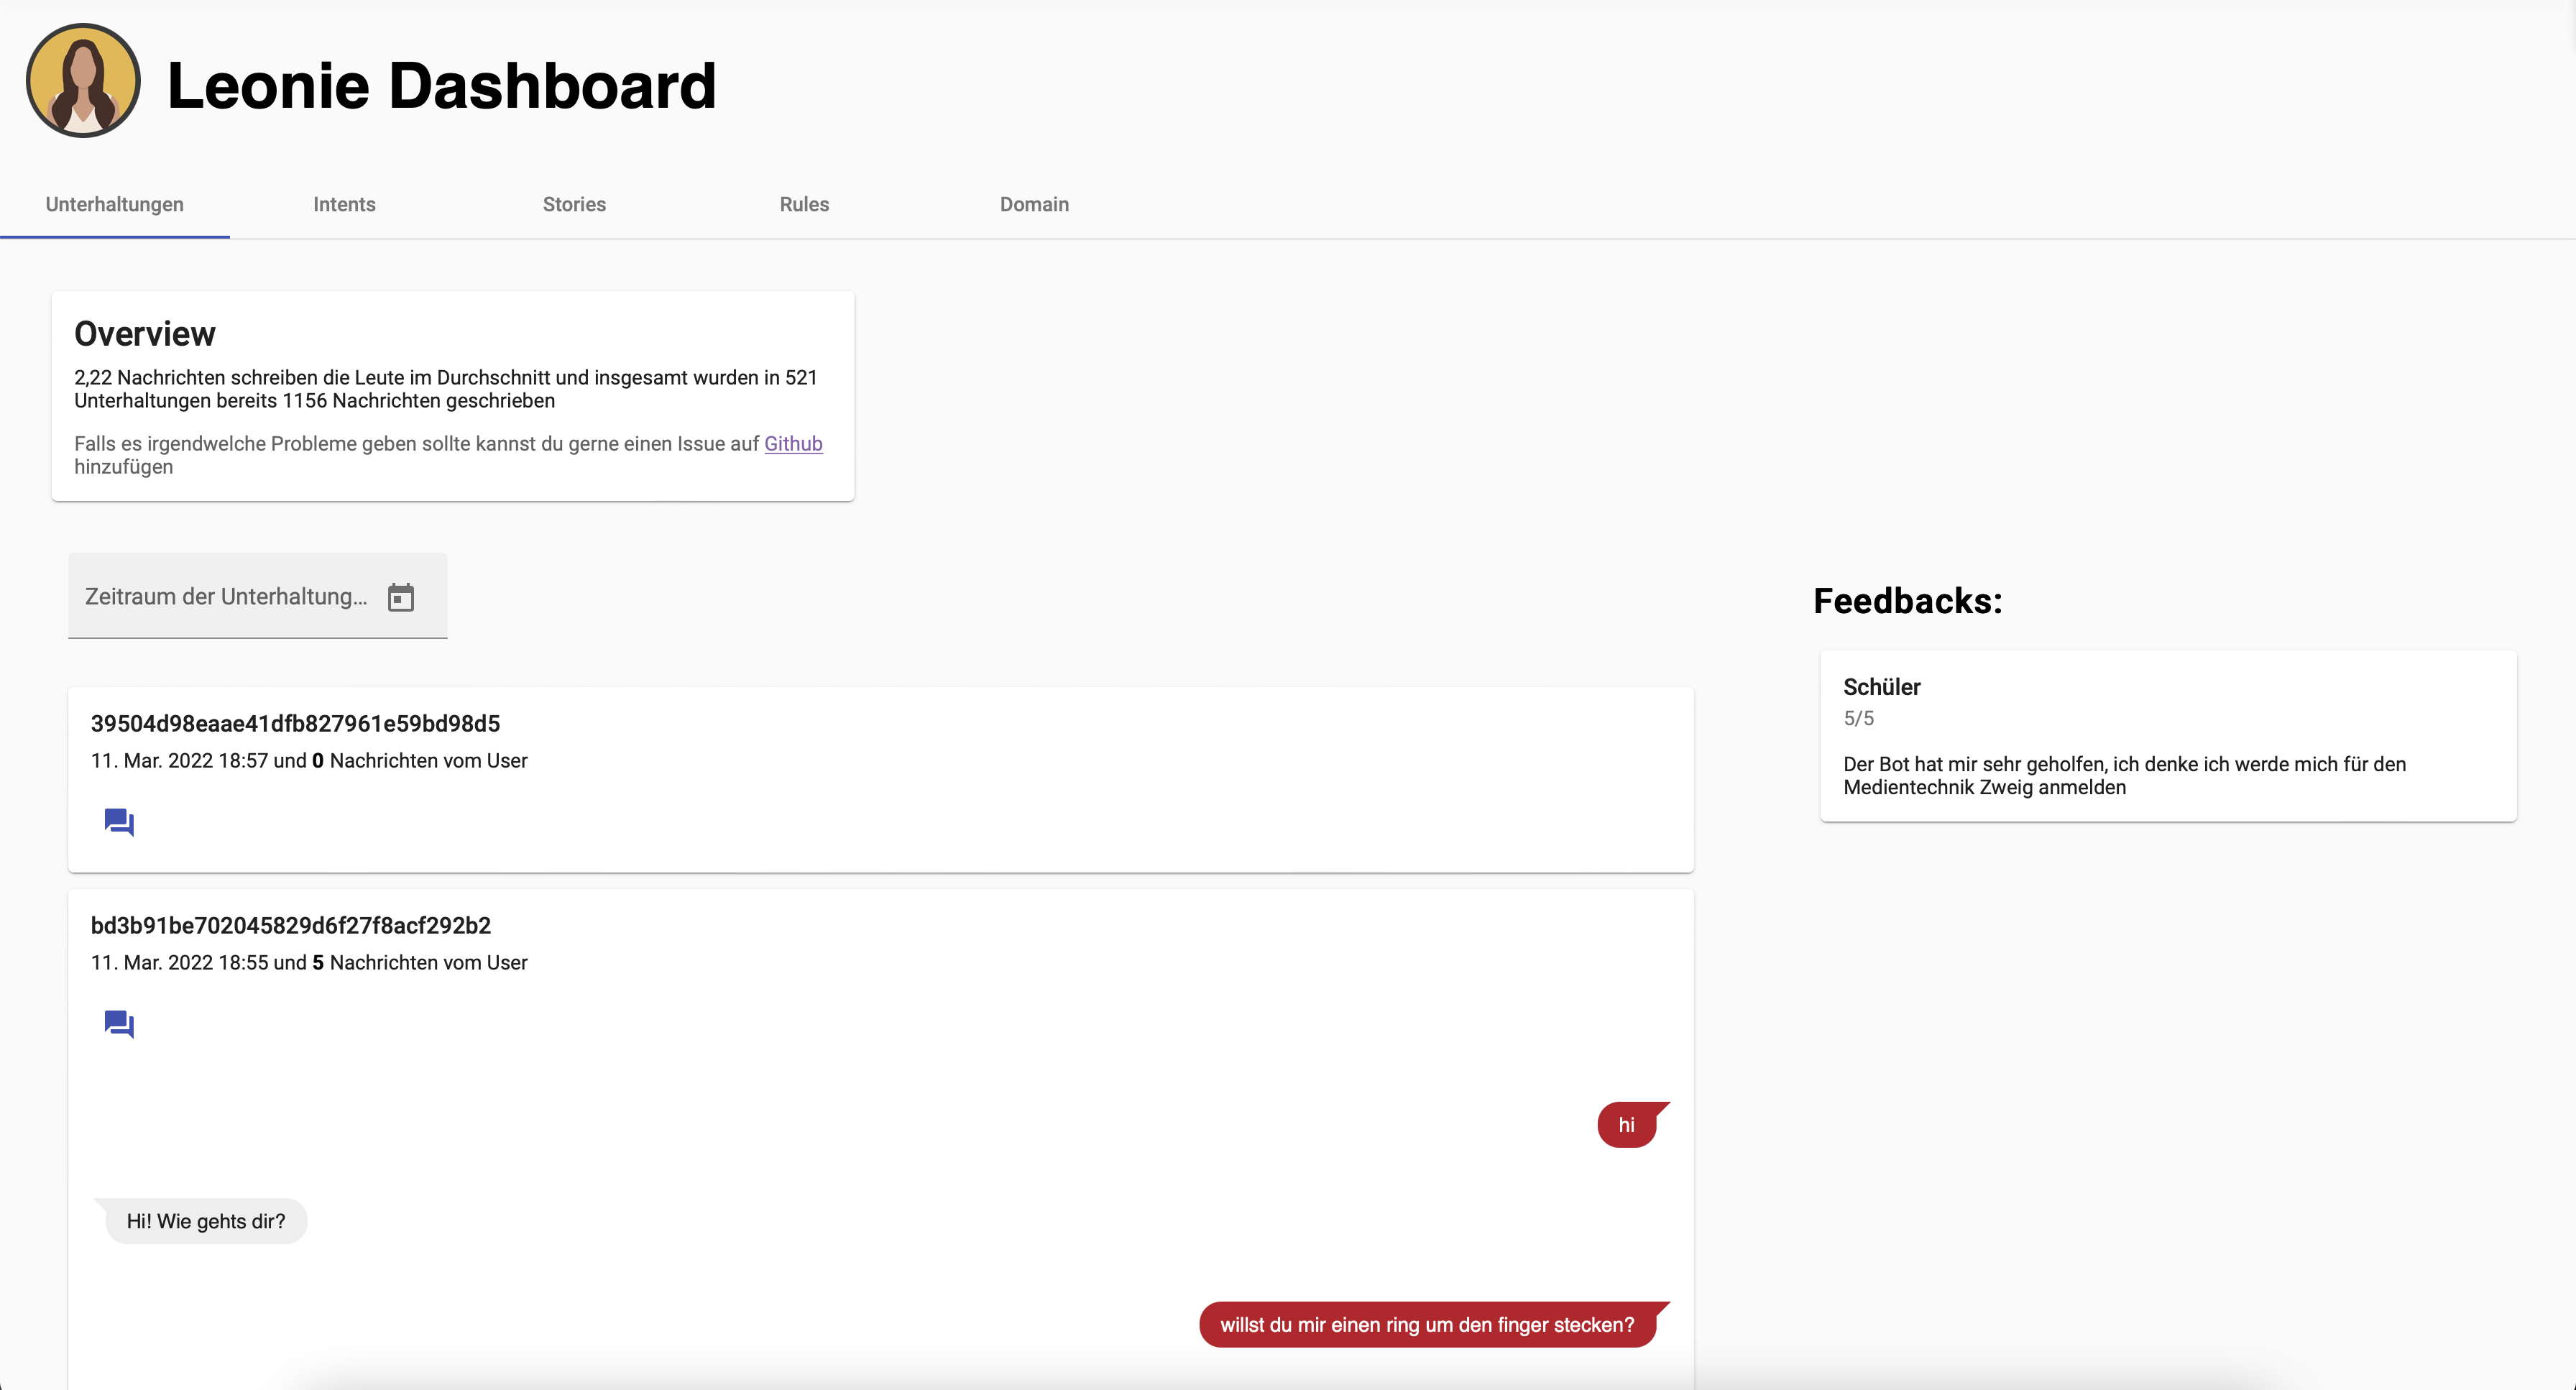
\includegraphics[scale=0.2]{pics/dashboardConvo}
    \caption{Dashboard}
    \label{fig:impl:dashConv}
\end{figure}

Die Unterhaltungen kann man zur Übersicht auch nach Datum filtern:

\begin{figure}[hbt!]
    \centering
    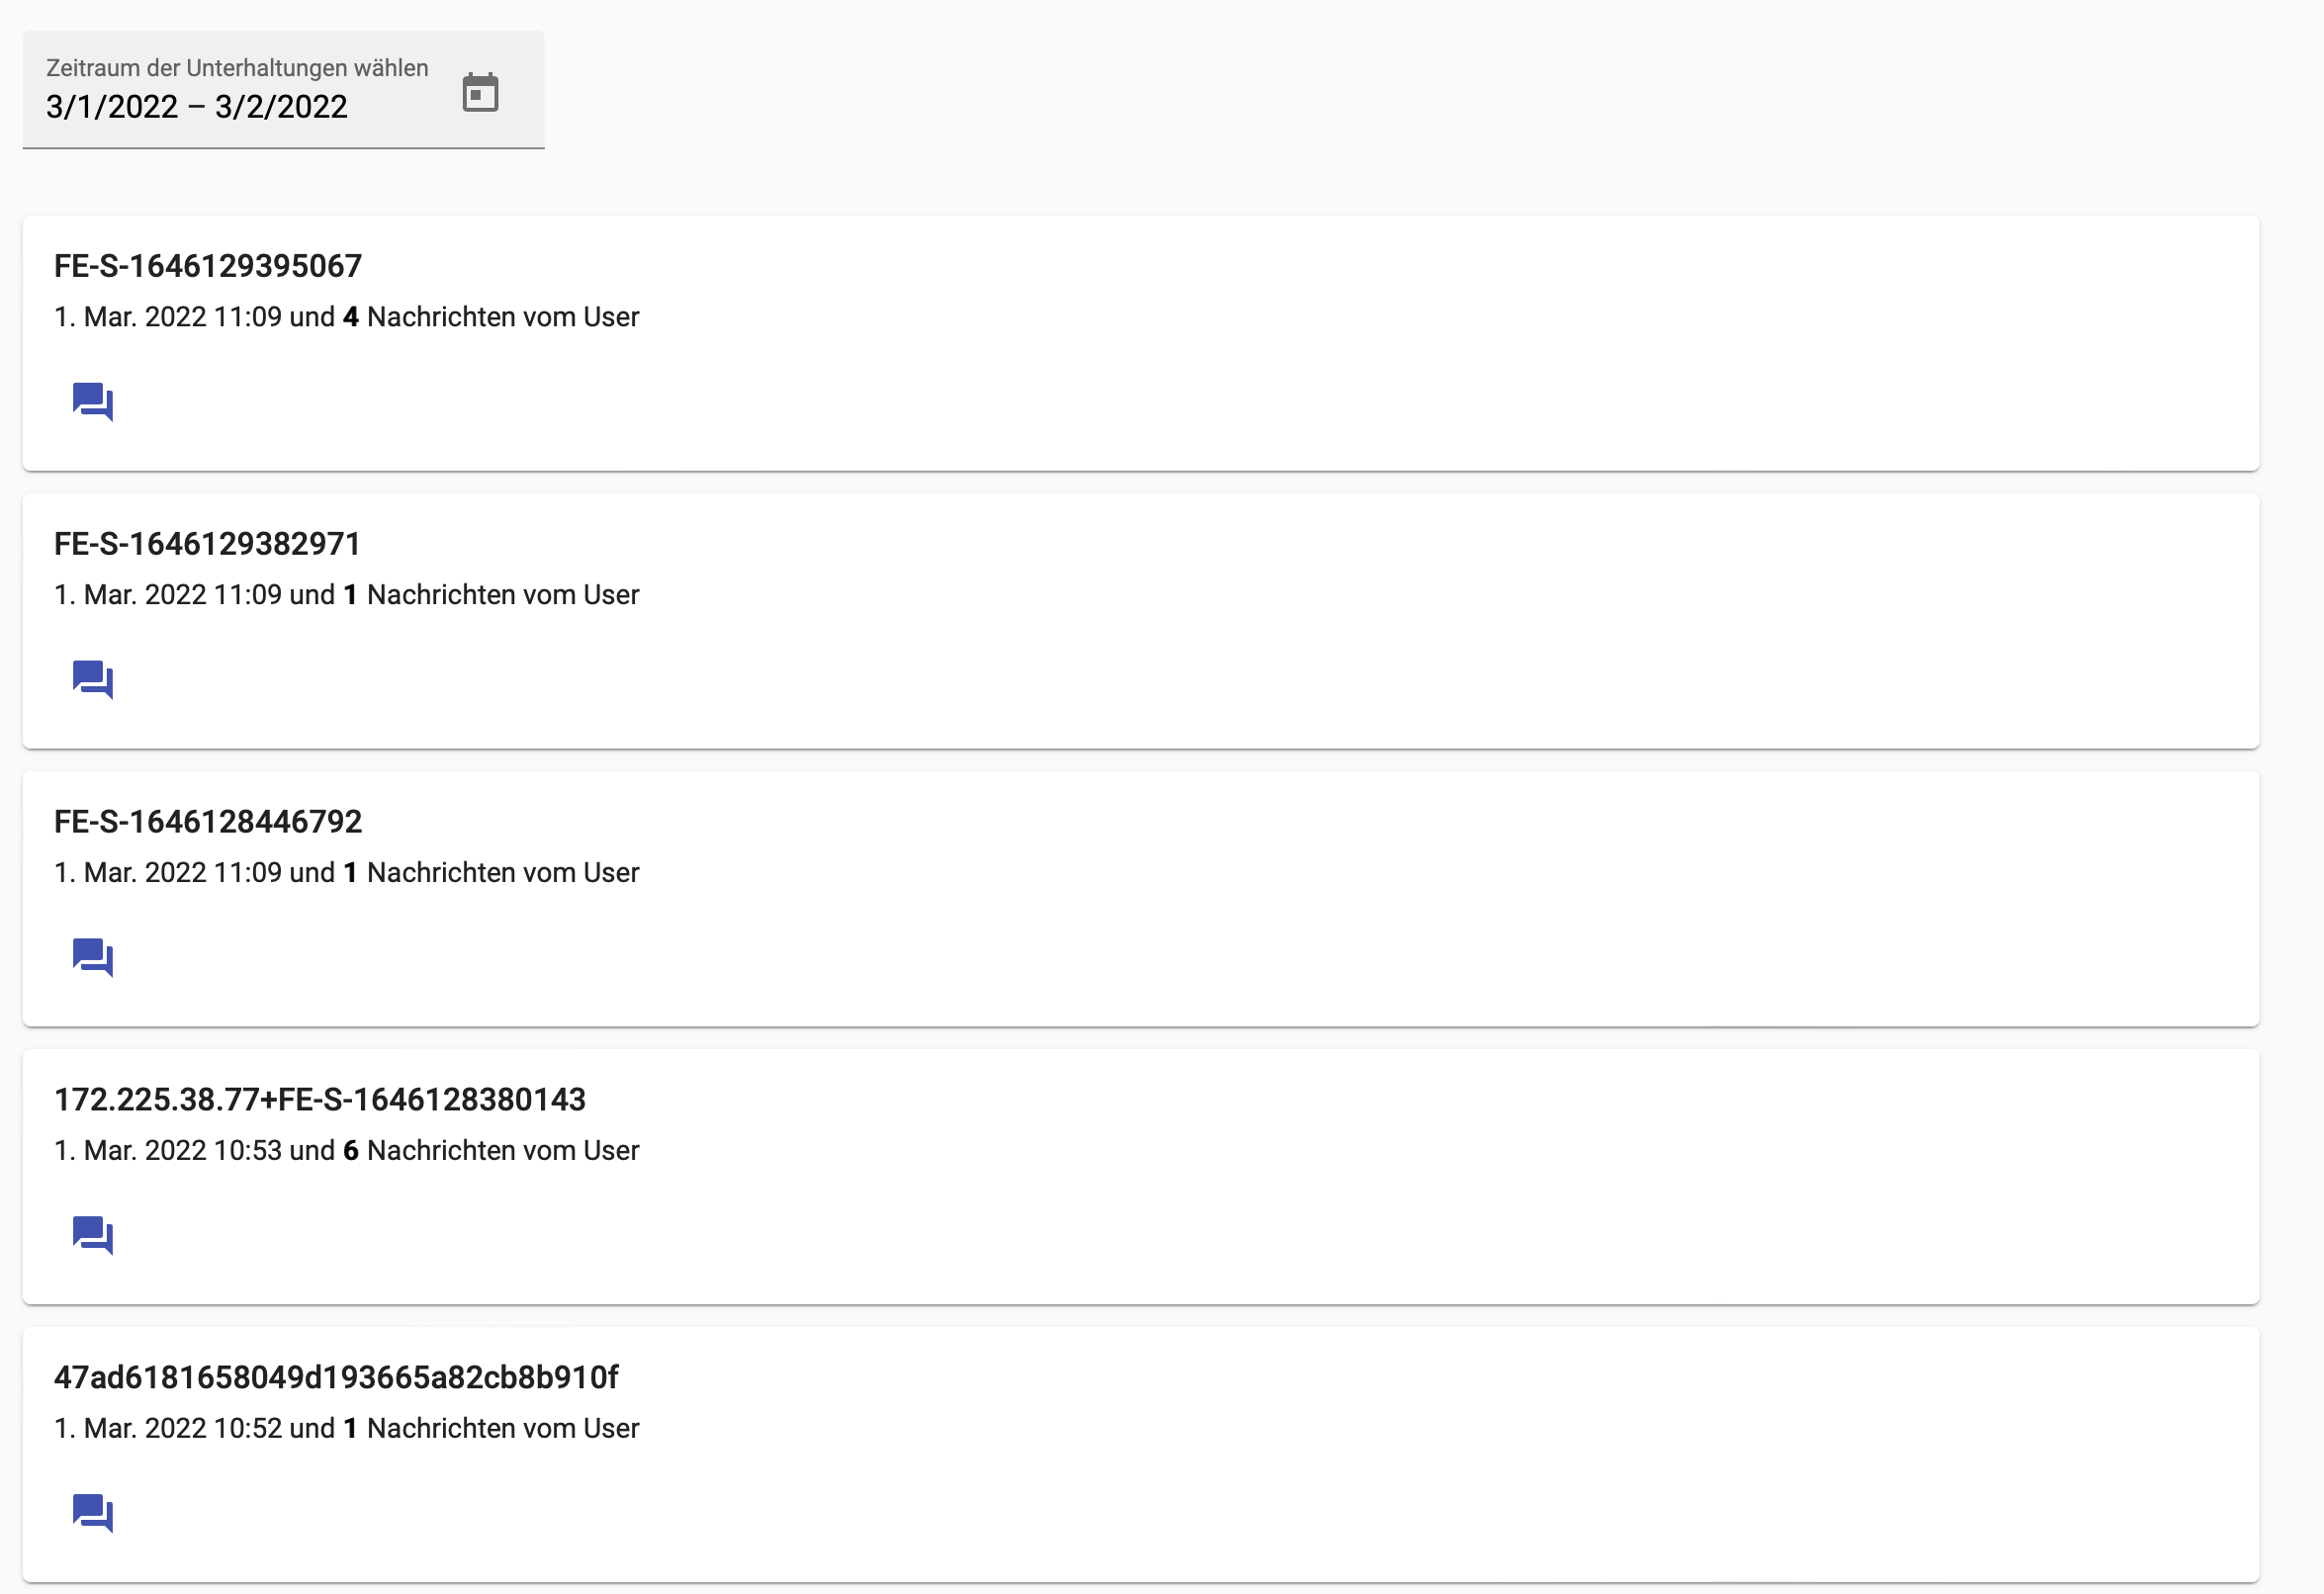
\includegraphics[scale=0.2]{pics/dashboardDate}
    \caption{Dashboard nach Datum gefiltert}
    \label{fig:impl:dashboardDate}
\end{figure}

Im Editor wurden auch Code Vorschläge benutzt um etwas an Tipparbeit sparen zu können.

\begin{figure}[hbt!]
    \centering
    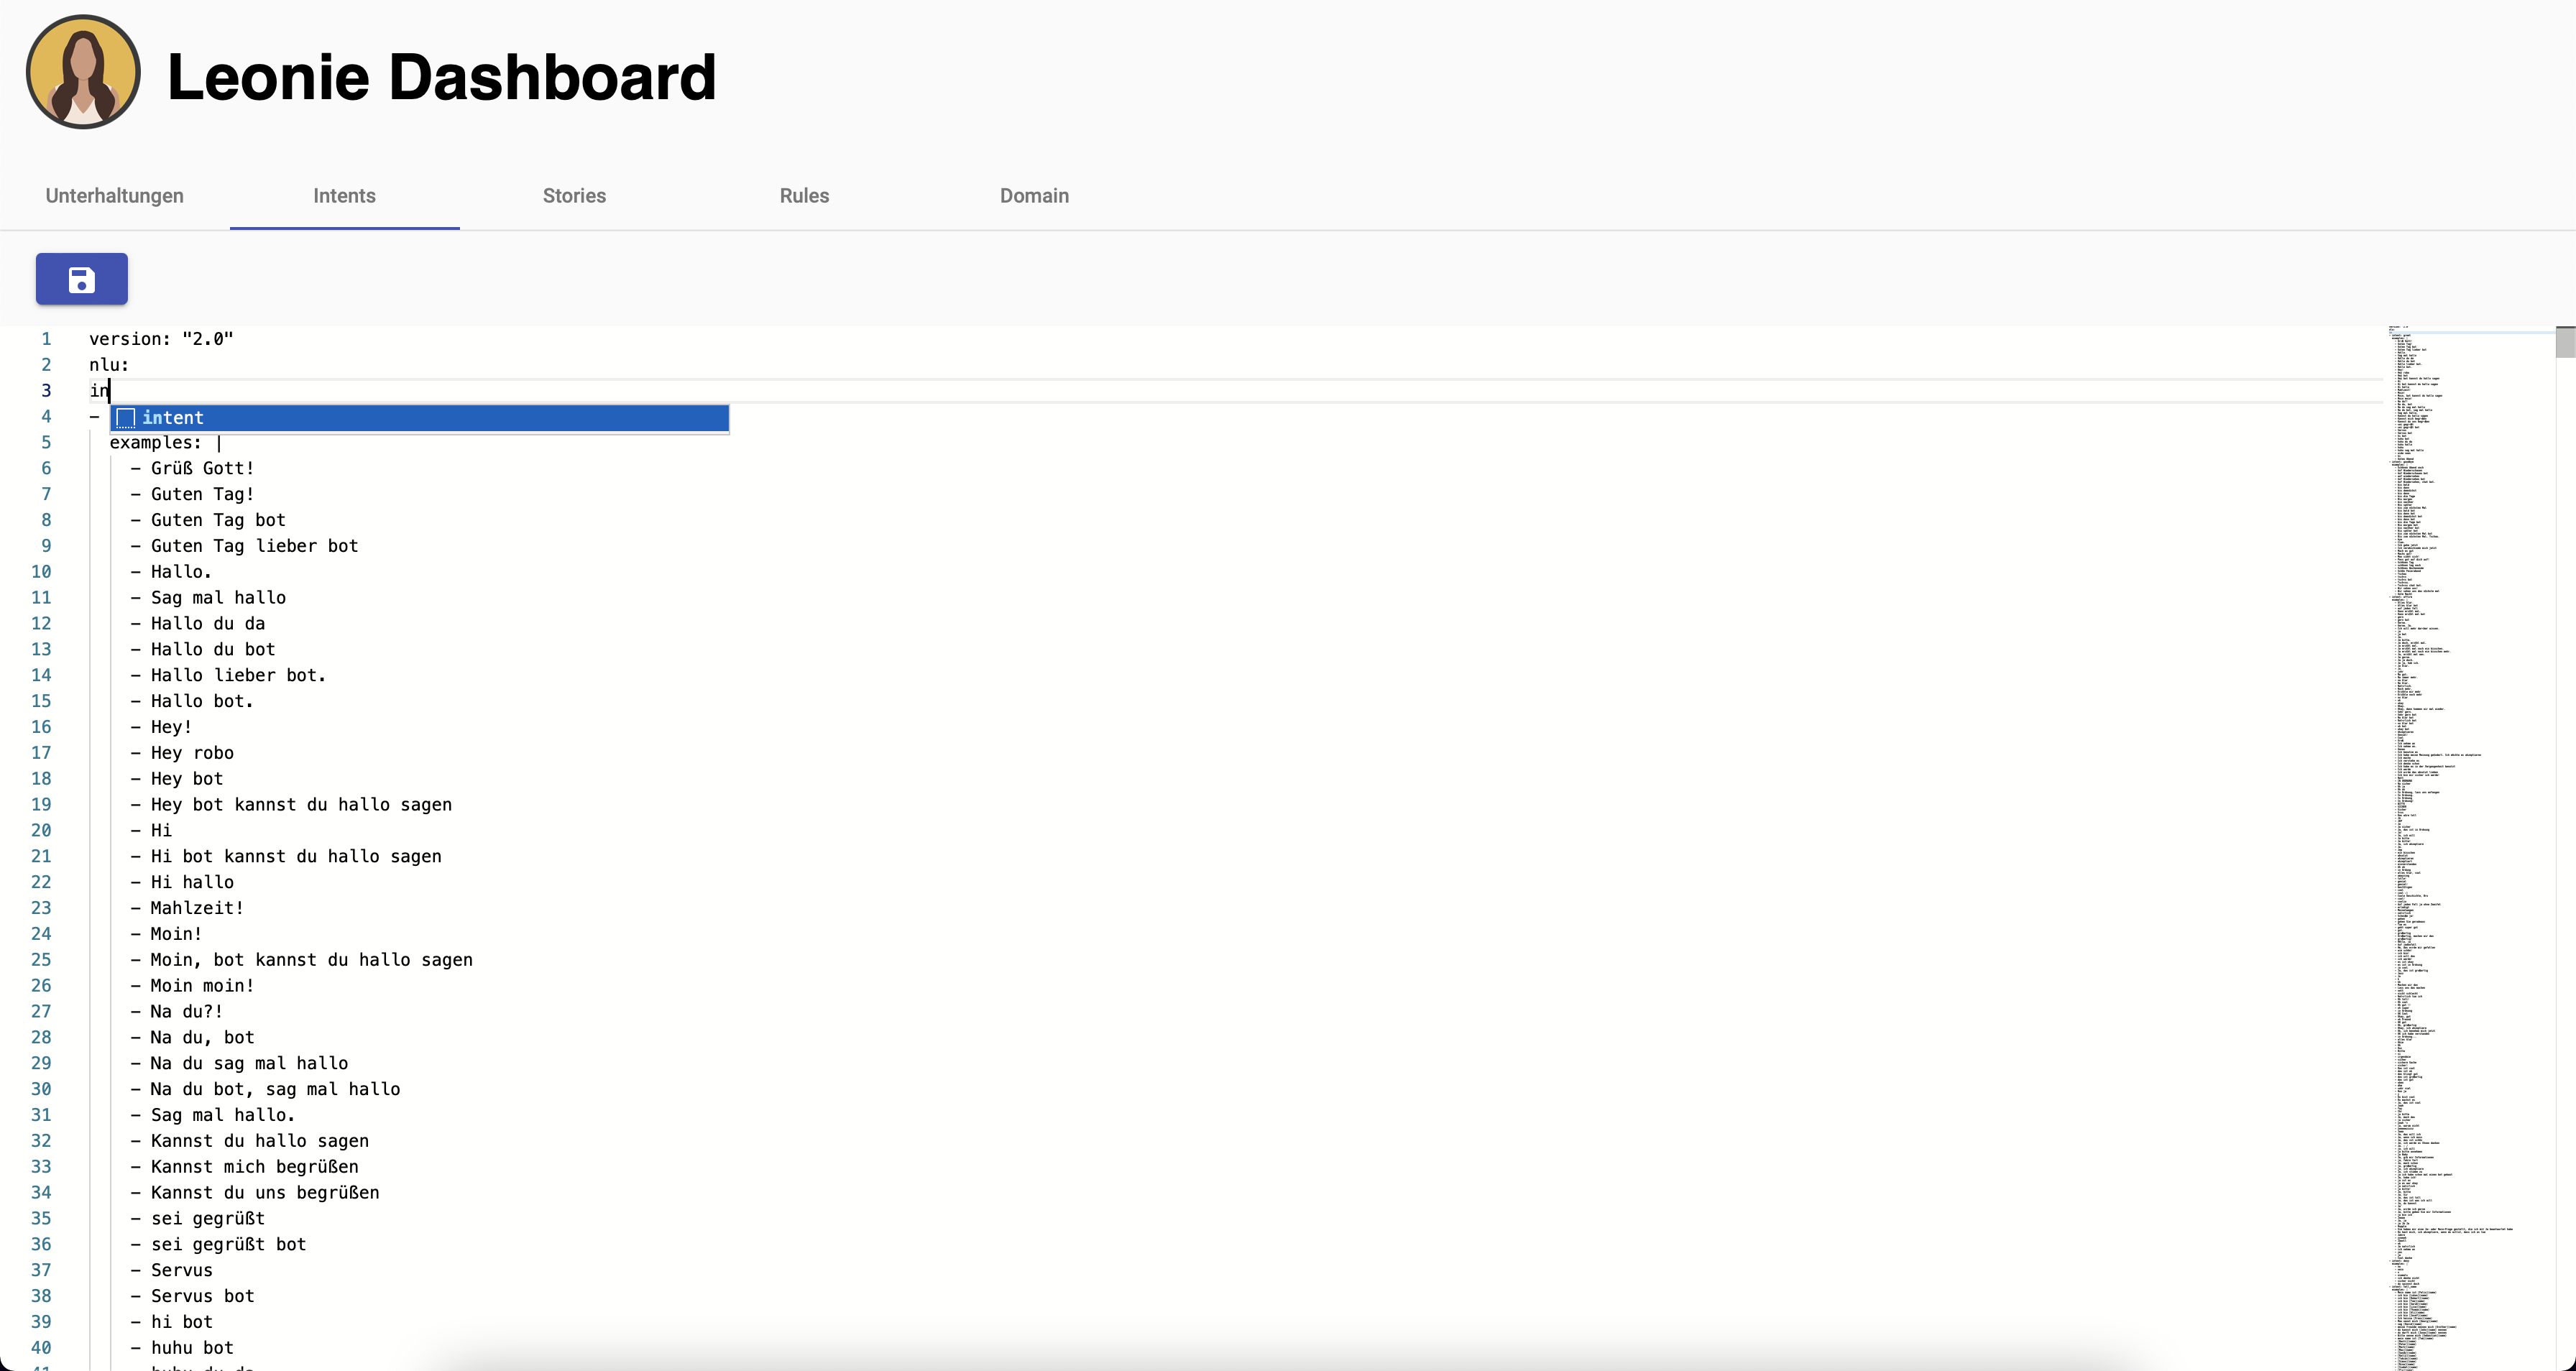
\includegraphics[scale=0.2]{pics/dashboardCodeSuggestion}
    \caption{Vorschläge}
    \label{fig:impl:dashboardCodeSuggestion}
\end{figure}
\begin{figure}[hbt!]
    \centering
    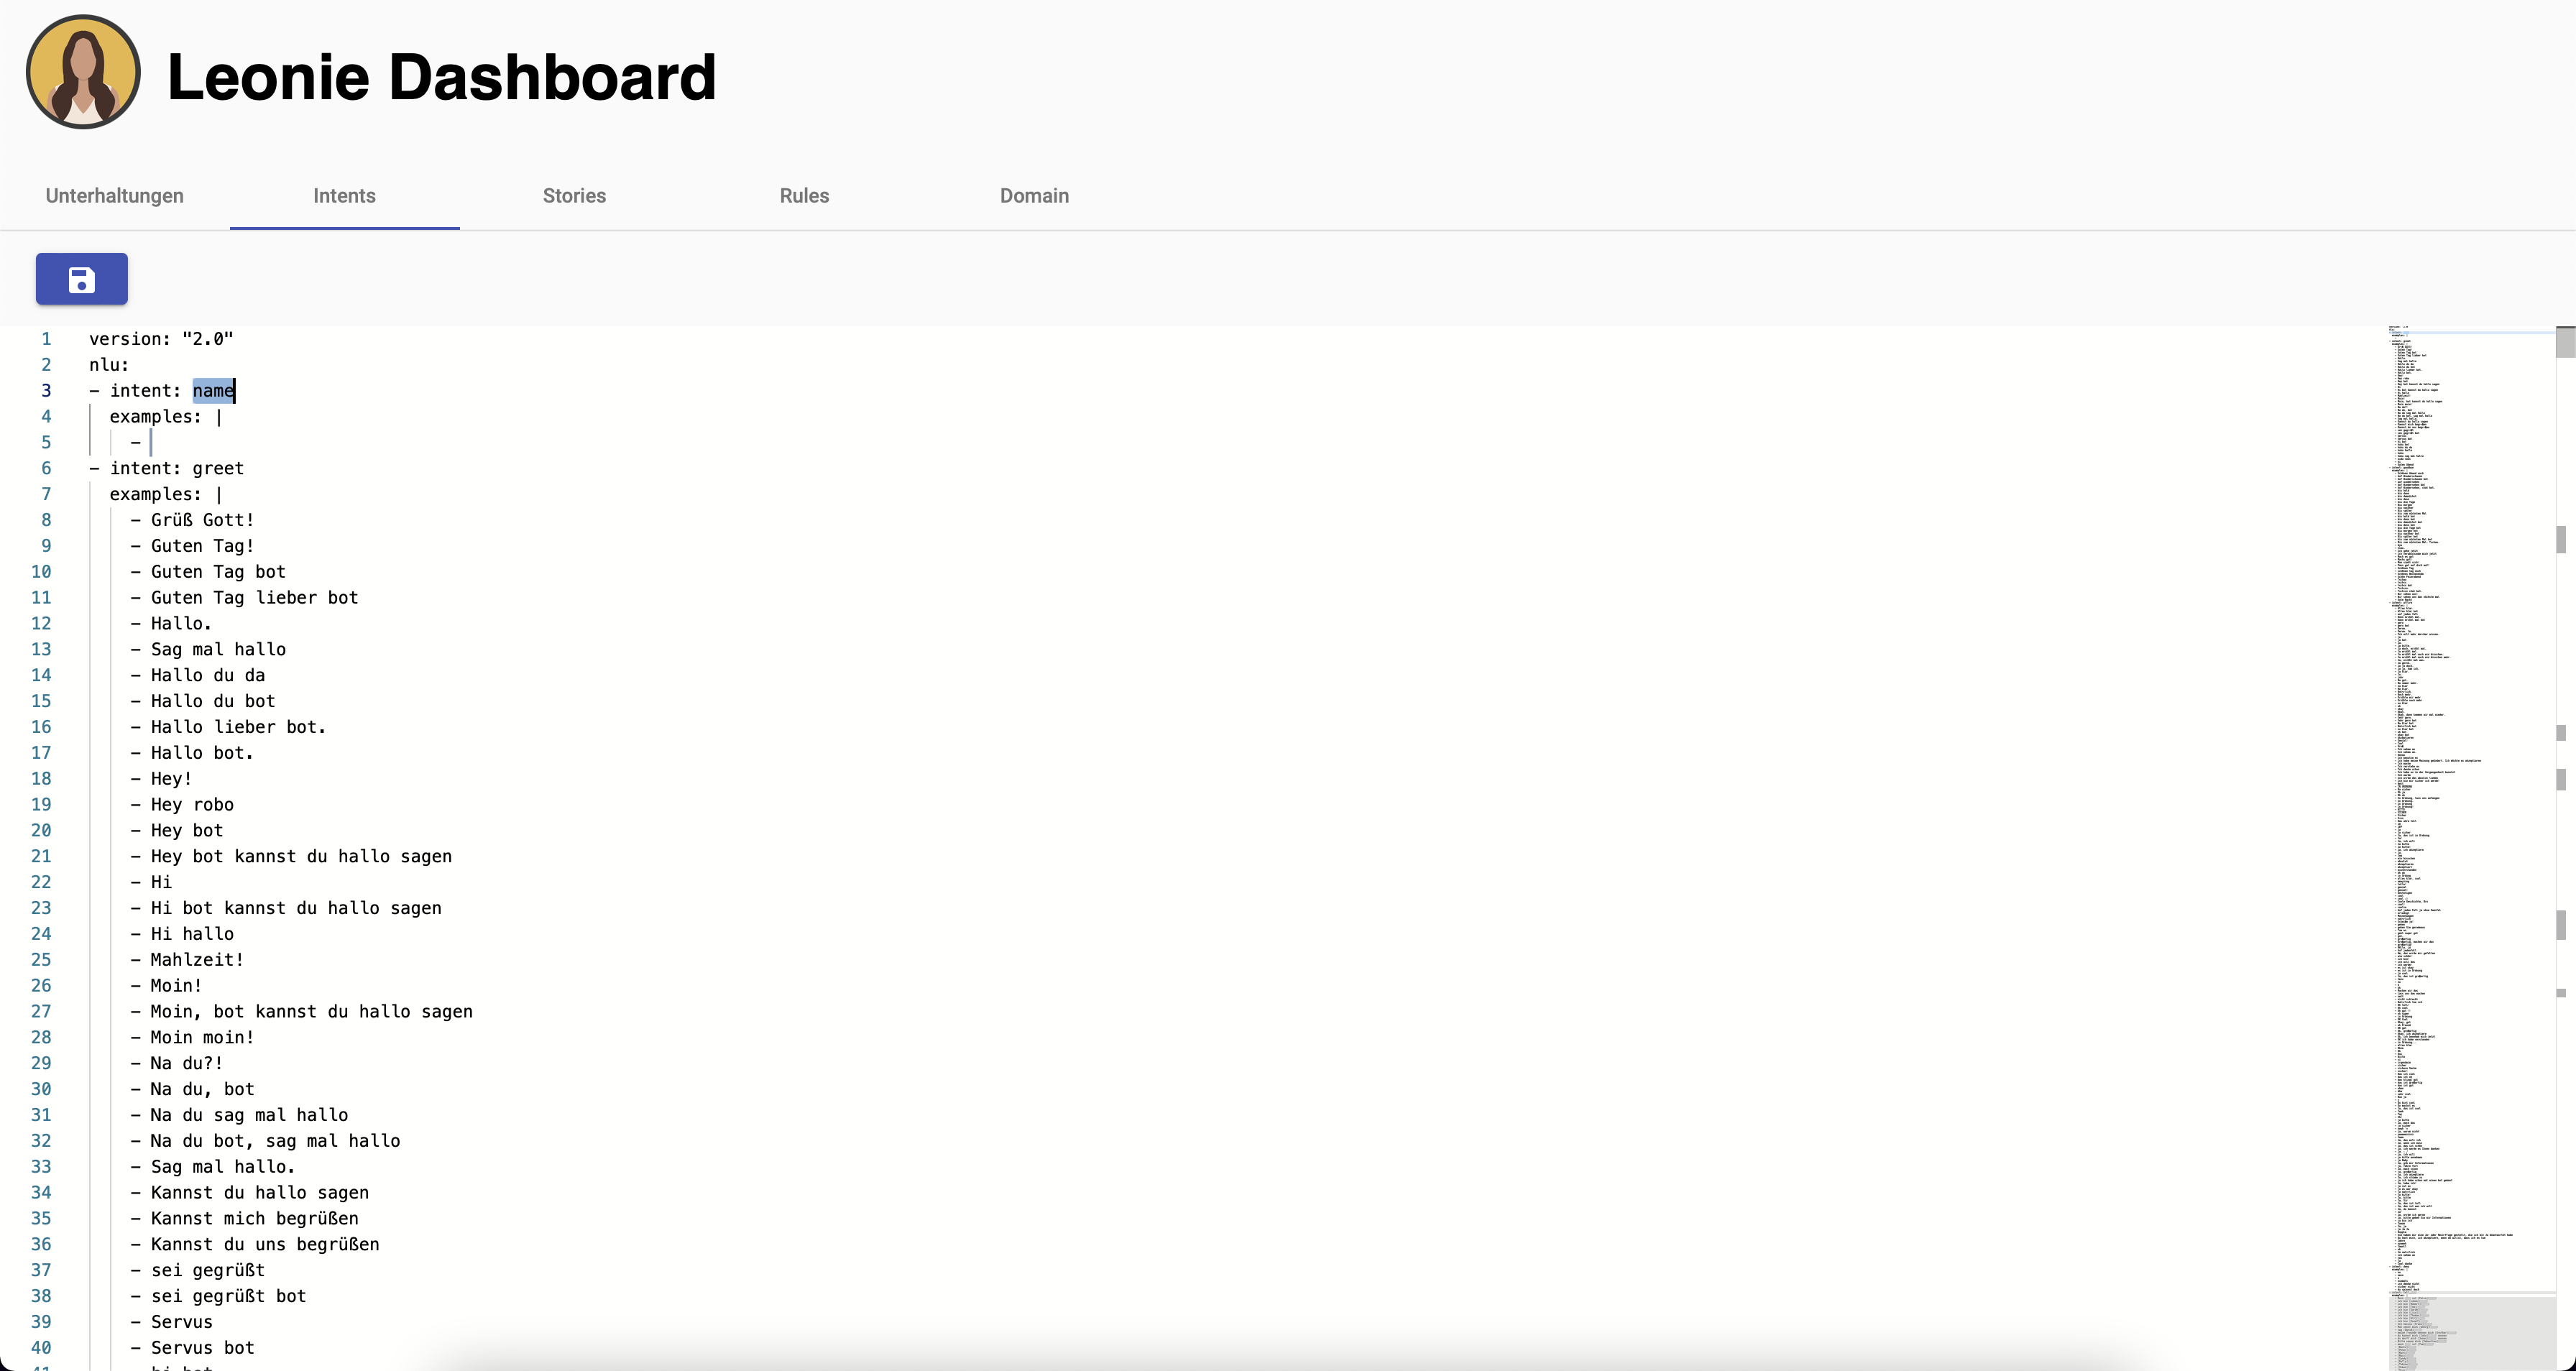
\includegraphics[scale=0.2]{pics/dashboardSuggestionMade}
    \caption{Vorschlag benutzt}
    \label{fig:impl:dashboardCodeSuggestionMade}
\end{figure}

Wir hoben uns für einen Editor entschieden und kein Fomular oder etwas ähnliches für die Verbesserung der Unterhaltungen, da ein Formular in dem Zustand das man den Bot so frei verändern kann wie mit dem Editor den Rahmen der Diplomarbeit gesprengt hätte.

\section{Einbindung in Wordpress}
Die HTL Leonding Webseite ist eine Wordpress Seite, deshalb musste der Chatbot als Webkomponente mit Angular Elements\ref{subsec:angular-elements} exportiert werden dass er dort eingebunden werden kann.

Auf Wordpress wurde das Plugin ``Shortcoder''\cite{shortcoder} installiert, dieses ermöglicht es Code Teile zu speichern.
Im Shortcoder Menu wurde ein neuer Shortcode mit unserer Webkomponente erstellt.

\begin{figure}[hbt!]
    \centering
    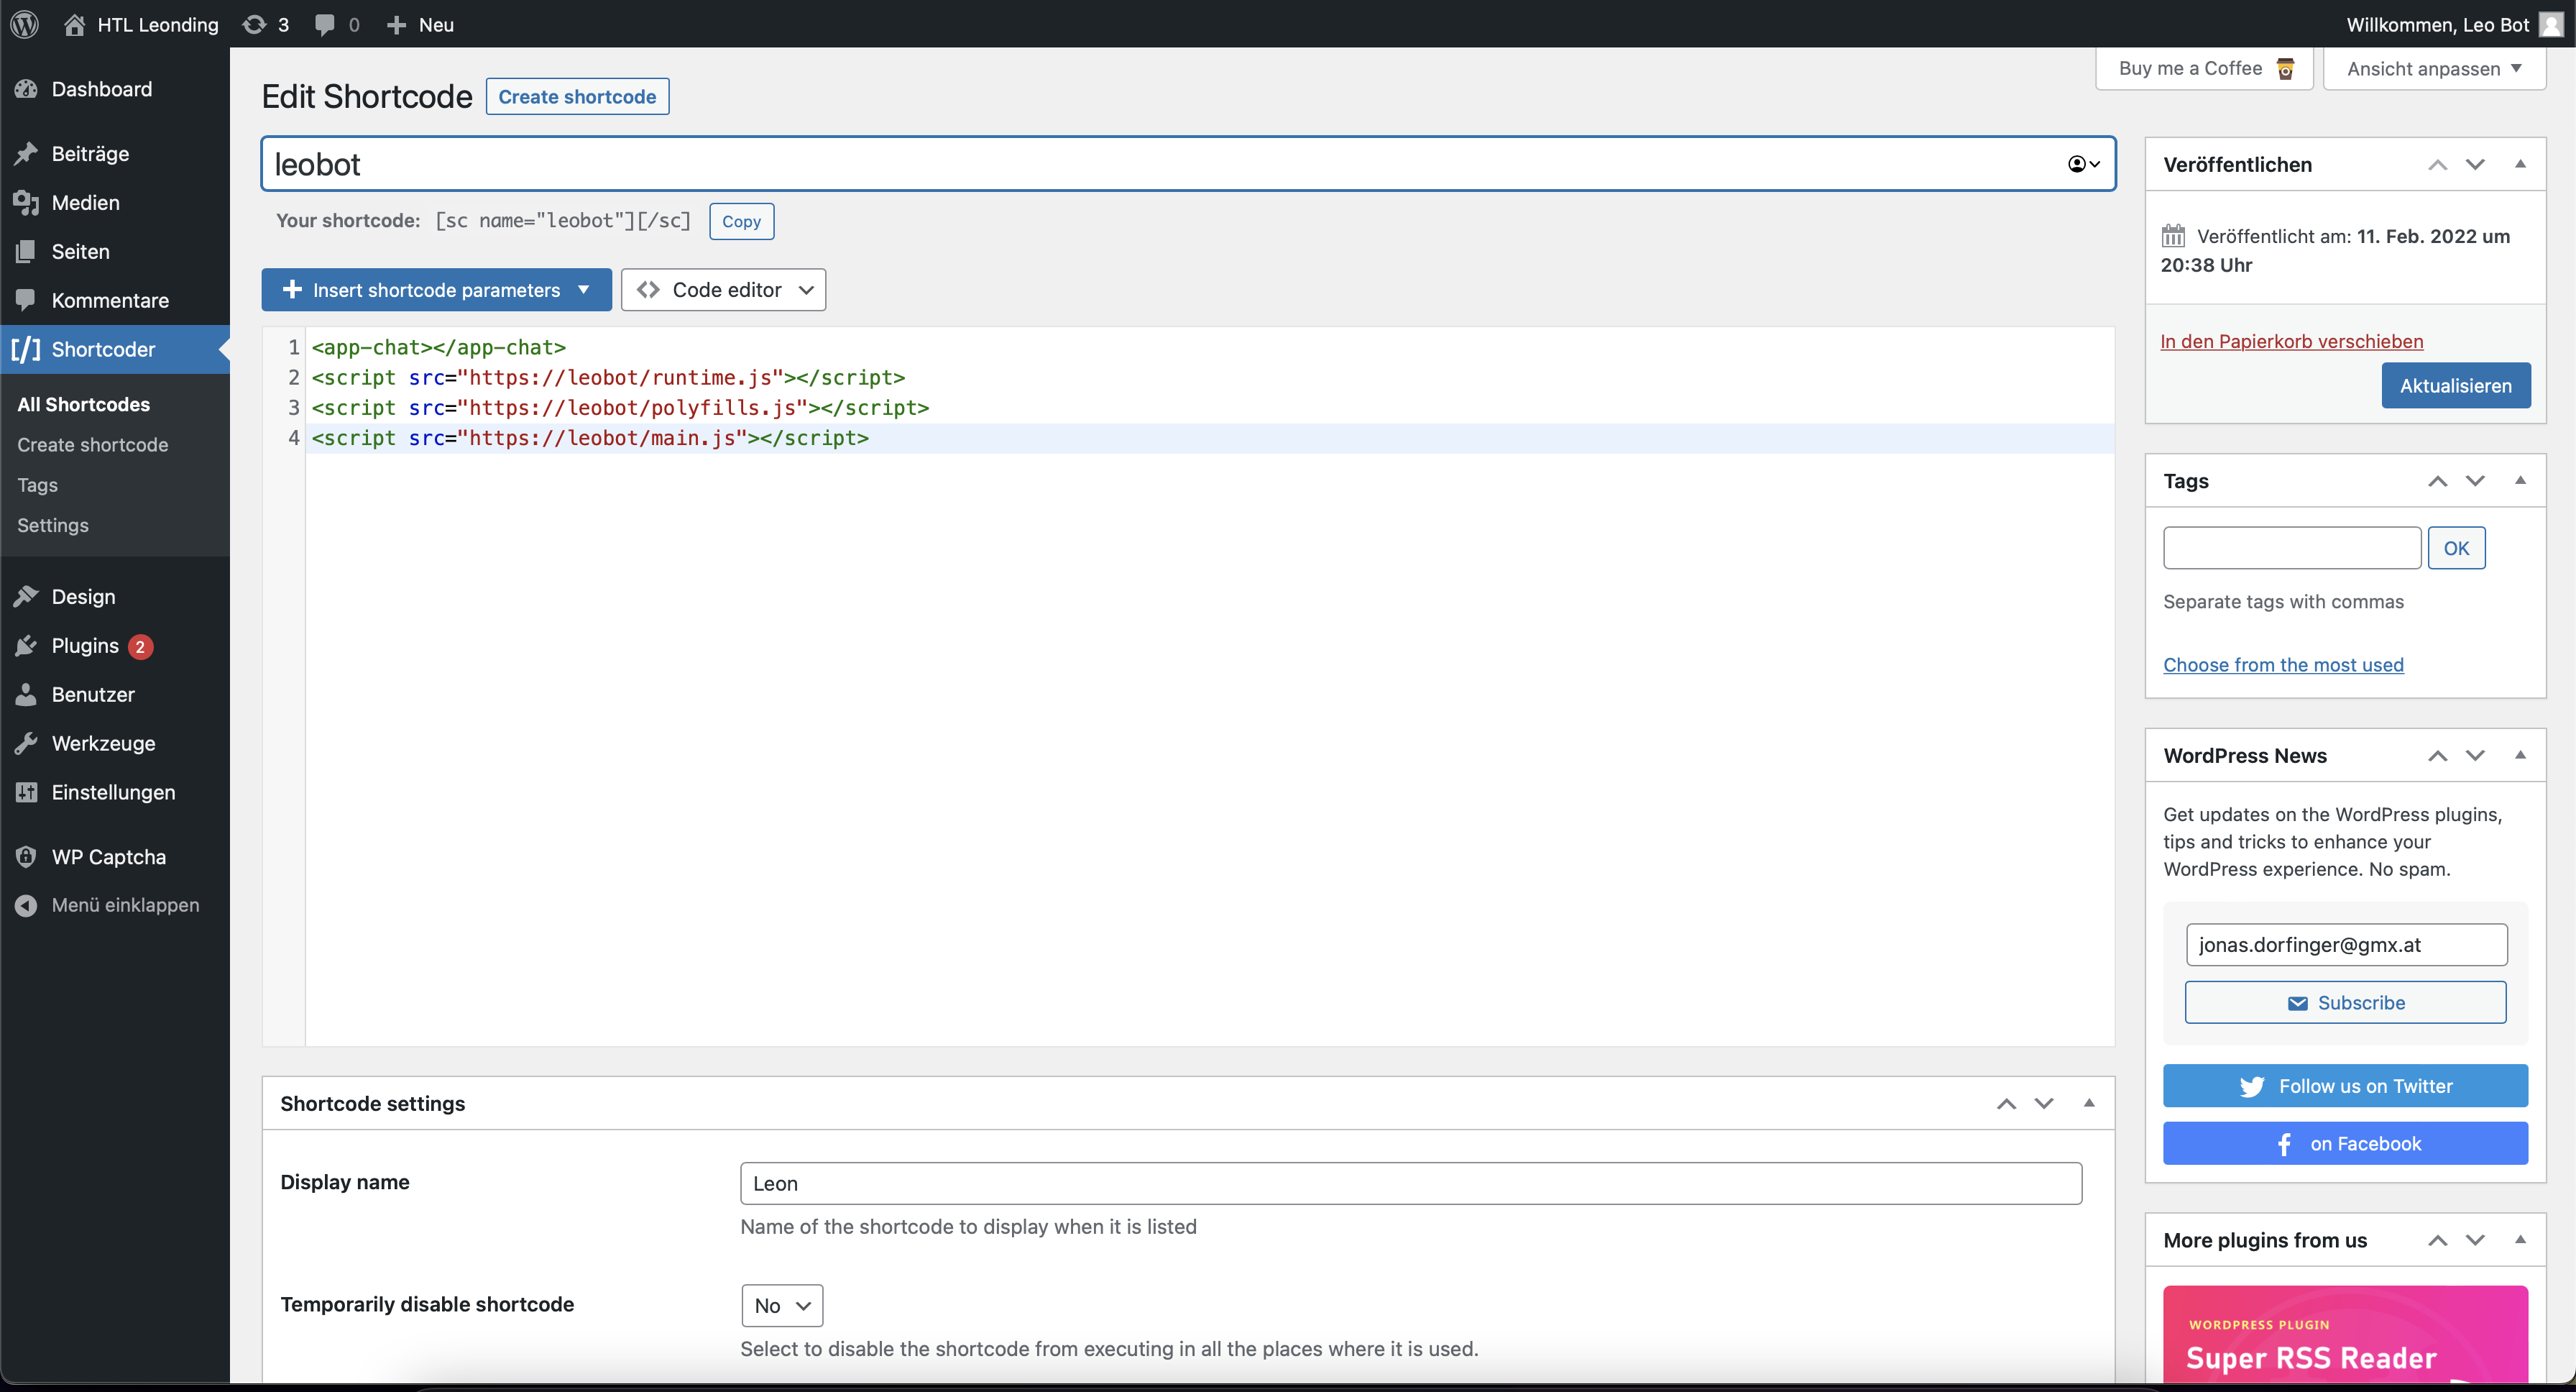
\includegraphics[scale=0.2]{pics/shortcoder}
    \caption{Shortcoder in Wordpress Plugin Manager}
    \label{fig:impl:shortcoder}
\end{figure}

Auf der Wordpress Seite wird nun der Shortcode eingefügt und somit der Chatbot eingebunden.

\begin{figure}[hbt!]
    \centering
    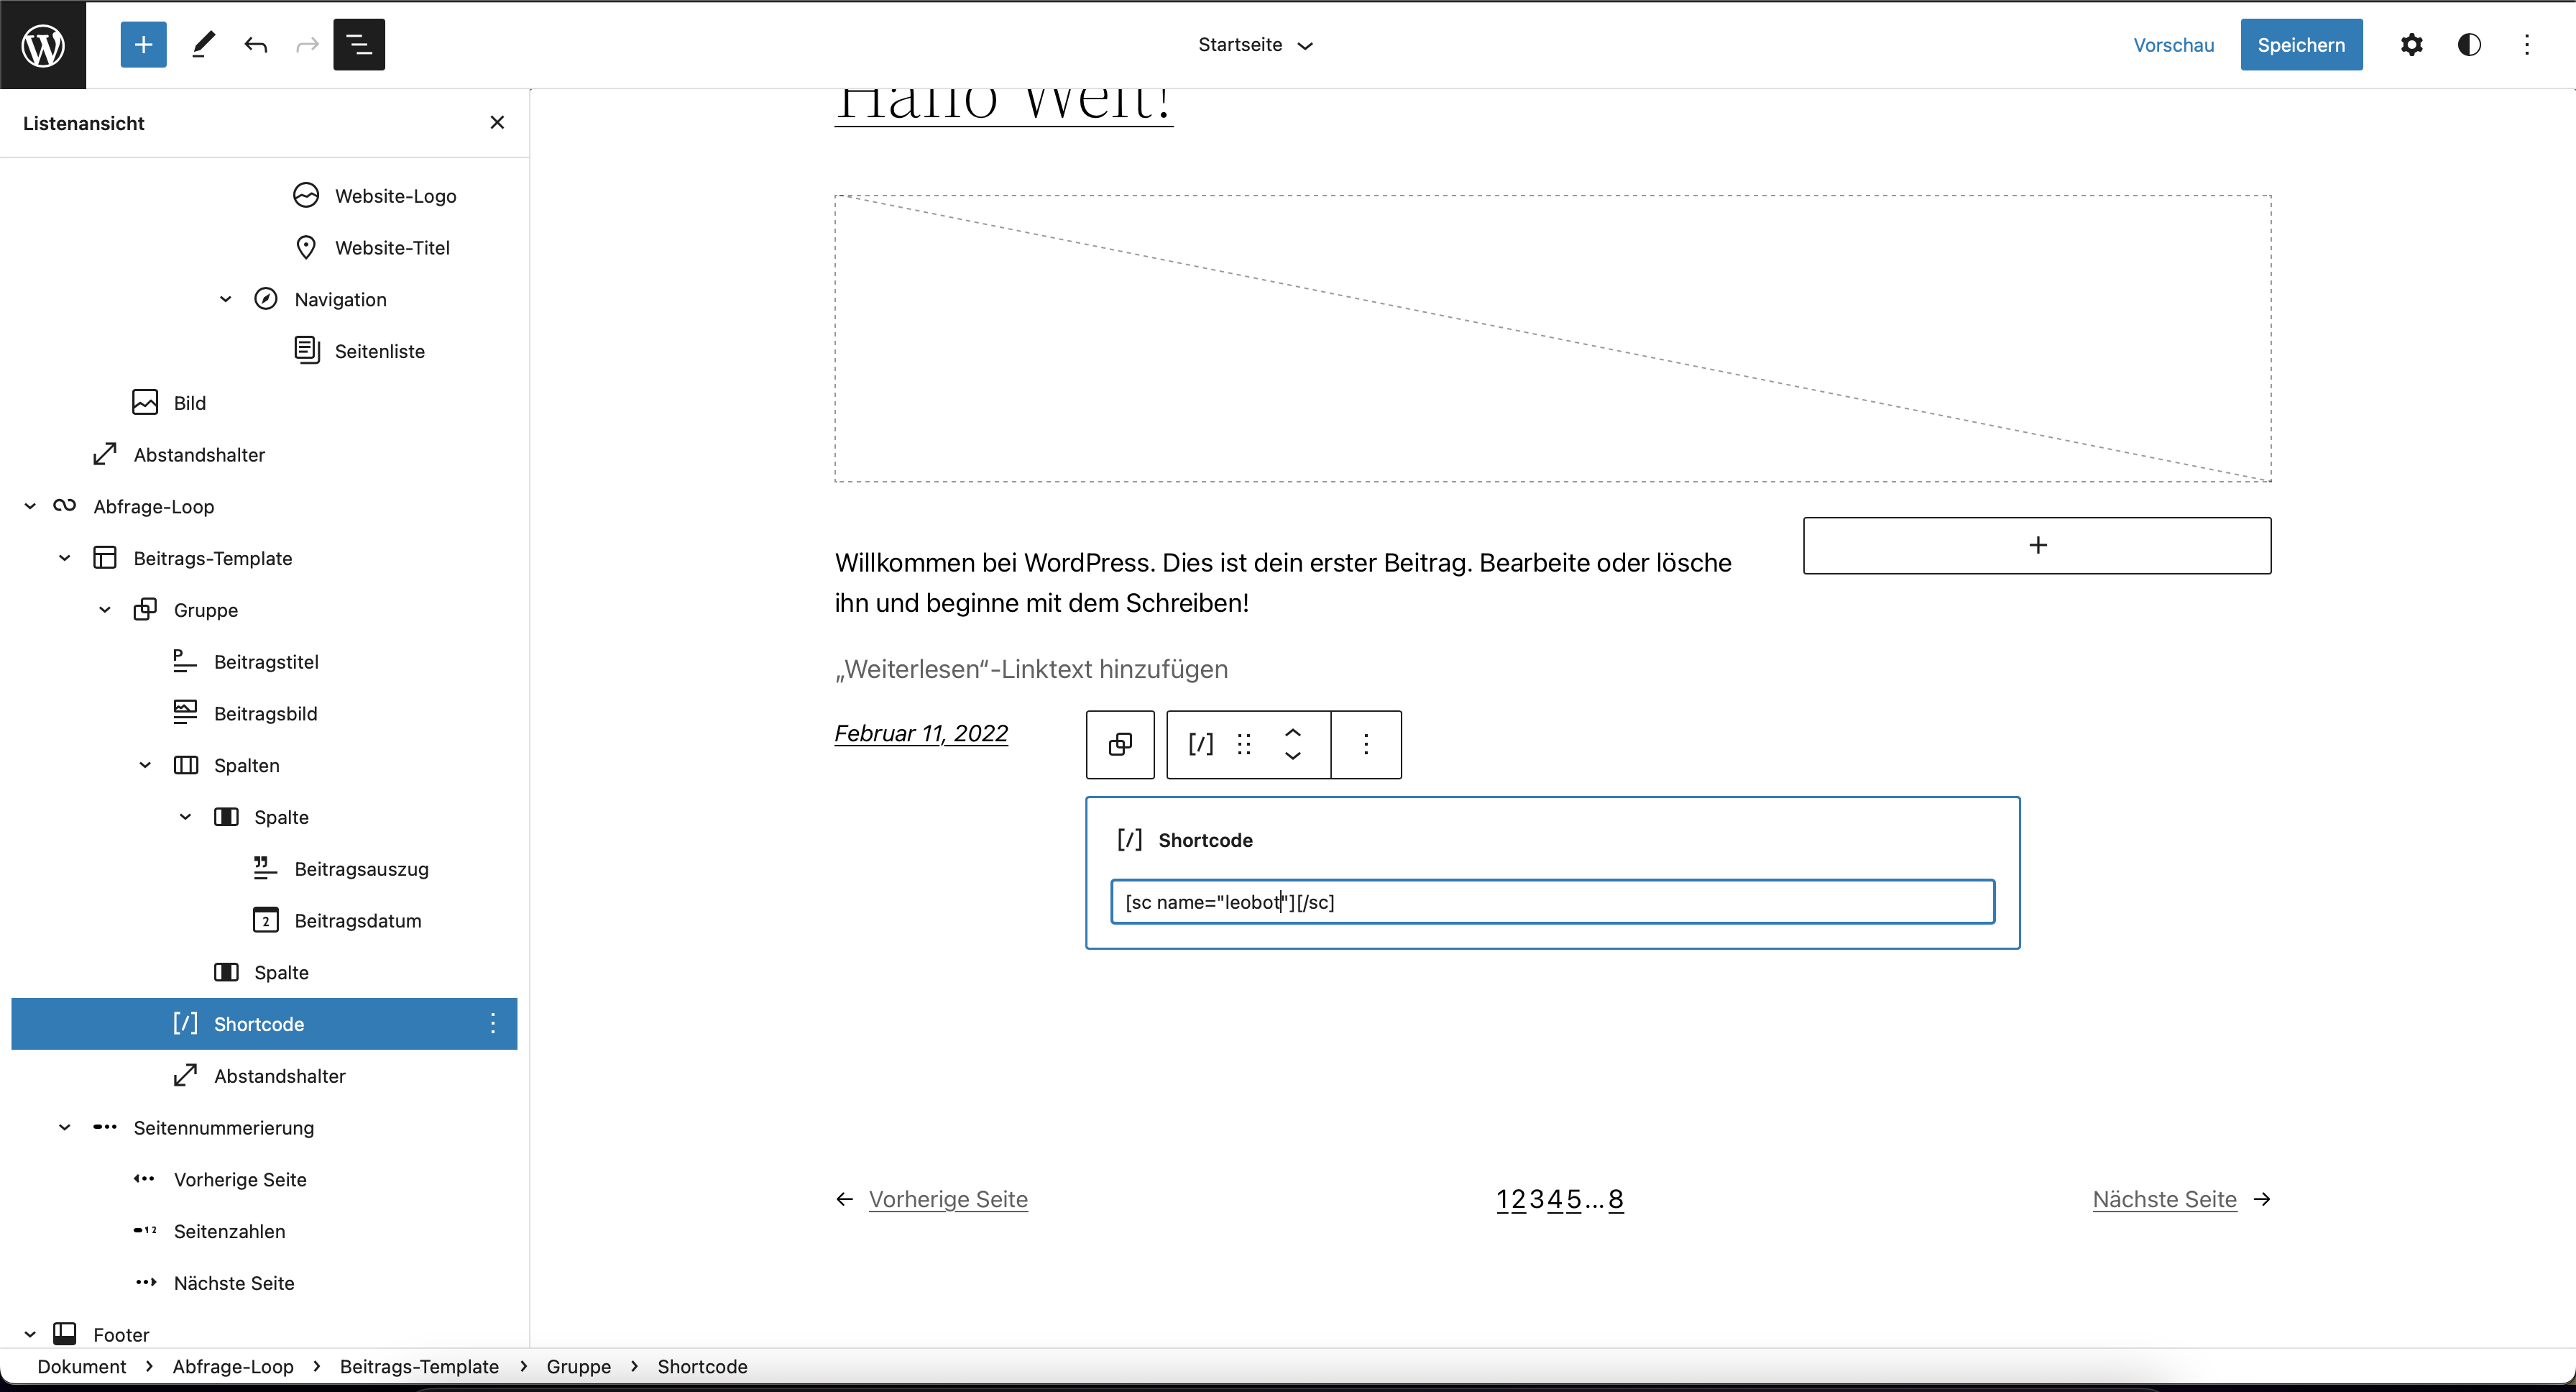
\includegraphics[scale=0.2]{pics/wordpressedit}
    \caption{Wordpress Editor}
    \label{fig:impl:wordpressedit}
\end{figure}

\begin{figure}[hbt!]
    \centering
    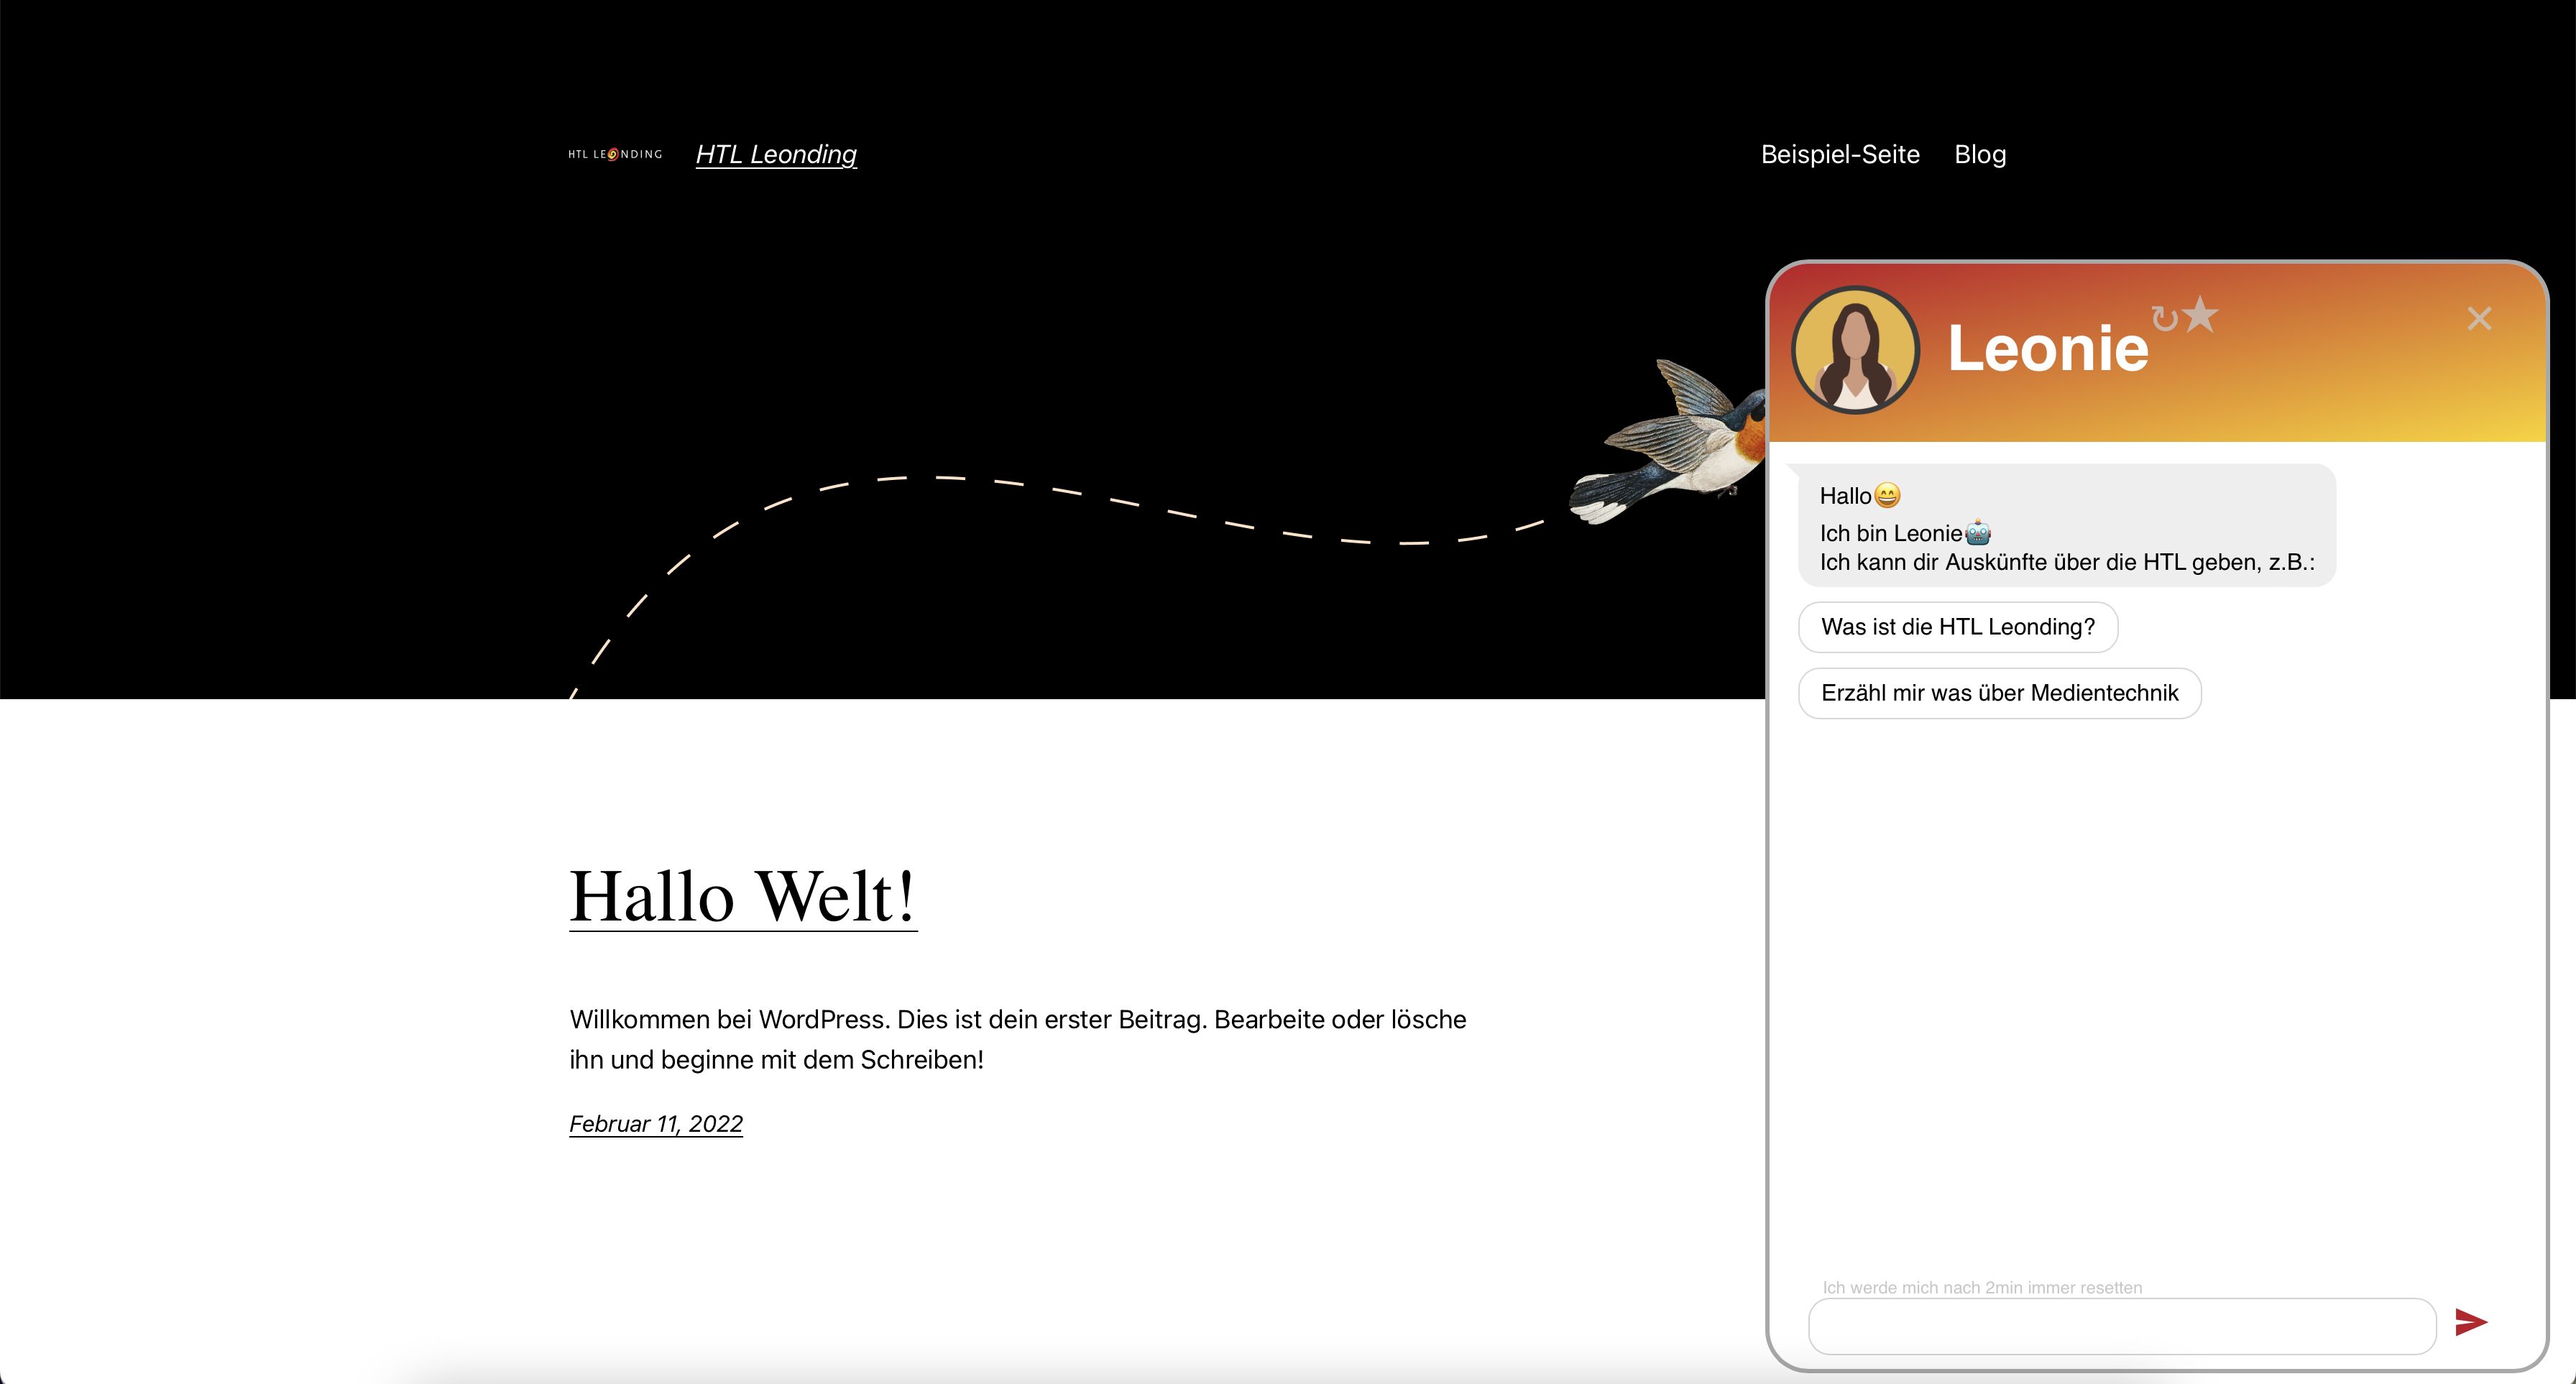
\includegraphics[scale=0.2]{pics/wordpresspage}
    \caption{Wordpress Seite mit Chatbot}
    \label{fig:impl:wordpresspage}
\end{figure}

\section{Deployment}

\subsection{GitHub Actions}

Die praktische Arbeit besteht aus sehr vielen einzelnen Projekten, wie dem Chat, Dashboard und Rasa selbst, diese haben alle verschiedenen Funktionen, bei vielen der GitHub Projekte wurde mithilfe von GitHub Actions\ref{subsec:github-actions} das Deployment automatisiert.

\subsubsection{Action Server}
Unser Rasa Custom Action Server wird mithilfe von GitHub Actions auf das LeoCloud Docker Registry geladen.

\begin{lstlisting}[language=yaml,label={lst:actionserveryml},caption={action\_server.yml}]{actionserver.yml}]
on:
  push:
    branches:
      - main
    paths:
    - 'rasa-docker-prototype/actions/**'

jobs:
  build_and_deploy:
    runs-on: ubuntu-latest
    name: Build Action Server image and upgrade Rasa X deployment
    steps:
    - name: Checkout repository
      uses: actions/checkout@v2

    - id: action_server
      name: Build an action server with a custom actions
      uses: RasaHQ/action-server-gha@main
      # Full list of parameters: https://github.com/RasaHQ/action-server-gha/tree/master#input-arguments
      with:
        actions_directory: 'rasa-docker-prototype/actions/'
        docker_registry: registry.cloud.htl-leonding.ac.at
        requirements_file: rasa-docker-prototype/actions/requirements.txt
        docker_image_name: 'f.dumfarth/leobot'
        docker_registry_login: ${{ secrets.LEO_LOGIN }}
        docker_registry_password: ${{ secrets.LEO_PASS }}
        # More details about github context:
        # https://docs.github.com/en/actions/reference/context-and-expression-syntax-for-github-actions#github-context
        #
        # github.sha - The commit SHA that triggered the workflow run
        docker_image_tag: 'leonie'
        docker_registry_push: true
\end{lstlisting}

Um den Action Server zu bauen, wird die ``RasaHQ/action-server-gha@main'' Action\cite{actionServerAction} benutzt.

Unsre genutzten Argumente sind:

%\begin{center}
%    \begin{tabular}{ |c|c| }
%        \hline
%        actions\_directory & Der Ordner in dem sich die Actions befinden \\
%        docker\_registry & Das Docker Registry wohin der Action Server hochgeladen werden soll \\
%        requirements\_file & Der Pfad zur requirements.txt Datei \\
%        docker\_image\_name & Der Name des Docker Images \\
%        docker\_registry\_login & Dein Username für das Docker Registry, am besten in einem Secret \\
%        docker\_registry\_password & Dein Passwort für das Docker Registry, am besten in einem Secret \\
%        docker\_image\_tag & der Tag des Docker Images \\
%        docker\_registry\_push & True oder False ob das Docker Image auf das Docker Registry hochgeladen werden soll \\
%        \hline
%    \end{tabular}
%\end{center}

\begin{itemize}
    \item actions\_directory: Der Ordner in dem sich die Actions befinden.
    \item docker\_registry: Das Docker Registry wohin der Action Server hochgeladen werden soll.
    \item requirements\_file: Der Pfad zur requirements.txt Datei.
    \item docker\_image\_name: Der Name des Docker Images.
    \item docker\_registry\_login: Dein Username für das Docker Registry, am besten in einem Secret.
    \item docker\_registry\_password: Dein Passwort für das Docker Registry, am besten in einem Secret.
    \item docker\_image\_tag: der Tag des Docker Images.
    \item docker\_registry\_push: True oder False ob das Docker Image auf das Docker Registry hochgeladen werden soll.
\end{itemize}

Auf der VM im docker-compose.yml muss noch das Image angeben:
\begin{lstlisting}[language=yaml,label={lst:dockercomposeyml},caption={docker-compose.yml}]{docker-compose.yml}]
app:
restart: always
image: "registry.cloud.htl-leonding.ac.at/f.dumfarth/leobot:leon"
expose:
- "5055"
depends_on:
- rasa-production
\end{lstlisting}

Man sieht dass unser Image den Namen ``leobot'' und den tag ``leon'' bekommen hat.

\subsubsection{Backend}
Das Backend wird mithilfe von GitHub Actions automatisiert gebaut, der Workflow baut das .jar file und dieses wird dann über SSH auf unsre VM geladen.

\begin{lstlisting}[language=yaml,label={lst:ciyml},caption={ci.yml}]{ci.yml}]
name: Quarkus Codestart CI

on:
  push:
    branches: [ main ]
  pull_request:
    branches: [ main ]

jobs:
  build:
    runs-on: ubuntu-latest
    steps:
      - uses: actions/checkout@v2
      - name: Set up JDK 17
        uses: actions/setup-java@v2
        with:
          distribution: 'temurin'
          java-version: '17'
      - name: Build
        run: ./mvnw clean package -Dquarkus.package.type=uber-jar -B
      - name: install ssh key
        uses: webfactory/ssh-agent@v0.5.3
        with:
          ssh-private-key: ${{ secrets.SSH_SERVER_PRIVATE_KEY }}
      - name: create .ssh/known_hosts
        run: |
          ssh-keyscan -H -t rsa -v ${{ secrets.SERVER }}  >> ~/.ssh/known_hosts
      - name: copy binaries to vm
        run: |
          echo "Hallo ich bin hier"
          ls -l target/
          scp target/leon-1.0.0-SNAPSHOT-runner.jar ${{ secrets.SERVER_USER }}@${{ secrets.SERVER }}:
\end{lstlisting}

\subsubsection{Frontend}
Die Chat Seite sowie das Dashboard werden mithilfe von GitHub Actions automatisiert gebaut und auf GH Pages gepublished dies passiert mit dem Workflow im build-and-deploy.yml file:

\begin{lstlisting}[language=yaml,label={lst:buildanddeployyml},caption={build-and-deploy.yml}]{build-and-deploy.yml}]
name: deploy to gh-pages

on:
  push:
    branches:
      - 'main'

jobs:
  build:
    name: Build ⚙
    runs-on: ubuntu-latest
    steps:
      - name: Checkout
        uses: actions/checkout@v2
      - name: Use Node 12.x
        uses: actions/setup-node@v1
        with:
          node-version: '12.x'
      - name: Install dependencies
        run: npm i
      - name: Build
        run: npm run build
      - name: Archive build
        if: success()
        uses: actions/upload-artifact@v1
        with:
          name: dist
          path: dist
  deploy:
    name: Deploy 🚀
    runs-on: ubuntu-latest
    needs: build
    steps:
      - name: Checkout
        uses: actions/checkout@v1
      - name: Download build
        uses: actions/download-artifact@v1
        with:
          name: dist
      - name: Deploy to GitHub Pages
        uses: JamesIves/github-pages-deploy-action@releases/v3
        with:
          GITHUB_TOKEN: ${{ secrets.GITHUB_TOKEN }}
          BRANCH: gh-pages
          FOLDER: dist/LeoBotHtlLeonding
\end{lstlisting}

Diese Action hat zwei Jobs, und zwar ``build'' und ``deploy''.

Die verschiedenen Tasks in Build, laden zuerst eine Node Version herunter, installieren die Dependencies, builden das Angular Projekt und schließlich wird dist in die Github Actions Artifacts gespeichert.

Beim Deploy Task wird dist von den Artefakten  heruntergeladen und wird in den Zweig ``gh-pages'' des Repositories gespeichert.

\subsubsection{Rasa}
\setauthor{Felix Dumfarth}

Wenn in das GH Repo etwas gepushed wird, wird mithilfe einer GitHub Action Rasa trainiert und das Model auf die VM geladen.

\begin{lstlisting}[language=yaml,label={lst:rasadeployyml},caption={rasa\_deploy.yml}]{rasa\_deploy.yml}]
name: Deploy Rasa to vm

on:
  push:
    branches:
      - 'main'
    paths:
      - 'rasa-docker-prototype/**'
  pull_request:
    branches:
      - 'main'

  workflow_dispatch:

jobs:
  branch:
    name: Deploy 🚀
    runs-on: ubuntu-latest
    steps:
      - name: Checkout
        uses: actions/checkout@v1
      - name: Deploy to Branch
        uses: JamesIves/github-pages-deploy-action@releases/v3
        with:
          GITHUB_TOKEN: ${{ secrets.TOKEN }}
          BRANCH: rasa-chatbot
          FOLDER: rasa-docker-prototype
  tests:
    name: Train and Test Rasa
    runs-on: ubuntu-latest
    needs: branch
    steps:
      - uses: actions/checkout@v2
        with:
          ref: rasa-chatbot
      - name: Train and Test Rasa
        uses: RasaHQ/rasa-train-test-gha@main
        with:
          test_type: all
          rasa_version: 2.8.12-full
          data_validate: true
          test_args: --fail-on-prediction-errors
          rasa_train: true
          rasa_test: true
      - name: Upload model
        uses: actions/upload-artifact@master
        with:
          name: model
          path: models
  deploy:
    name: "Deploy to vm"
    runs-on: ubuntu-latest
    needs: tests
    steps:
      - name: Download model
        uses: actions/download-artifact@v2
        with:
          name: model
          path: models
      - name: Copy model to vm
        uses: garygrossgarten/github-action-scp@release
        with:
          local: models
          remote: /home/chatadm/leobot/models
          host: ${{ secrets.SSH_HOST }}
          username: ${{ secrets.SSH_USER }}
          privateKey: ${{ secrets.SSH_KEY }}
      - name: Configure SSH
        run: |
          mkdir -p ~/.ssh/
          echo "$SSH_KEY" > ~/.ssh/staging.key
          chmod 600 ~/.ssh/staging.key
          cat >>~/.ssh/config <<END
          Host staging
            HostName $SSH_HOST
            User $SSH_USER
            IdentityFile ~/.ssh/staging.key
            StrictHostKeyChecking no
          END
        env:
          SSH_USER: ${{ secrets.SSH_USER }}
          SSH_KEY: ${{ secrets.SSH_KEY }}
          SSH_HOST: ${{ secrets.SSH_HOST }}
      - name: Copy model to Rasa X
        run: ssh staging 'cd /home/chatadm/leobot/models && ./upload-latest-model.sh'
\end{lstlisting}

Es wir zu erst geschaut ob der push wirklich auf den Branch ``main'' geschickt wurde und dort im Ordner ``raser-dokcer-prototype'' sich etwas verändert hat, wenn dies zutrifft wird der Workflow ausgeführt.

Im Job Branch wird zuerst der Ordner der mithilfe des ``FOLDER:'' Arguments angegeben wurde, also ``rasa-docker-prototype'' auf den BRACNH, der mit ``BRANCH:'' angegeben wurde, also ``rasa-chatbot'' geladen

Im Job tests wird zuerst definiert das der Job ``branch'' benötigt wird bevor tests ausgeführt werden kann, dies wird mit dem ``needs:'' Argument definiert.
Beim Checkout wird nun bei ``ref:'' der Branch angegeben, da wir nun mit dem, auf den zuvor gepushed, Branch ``rasa-chatbot'' arbeiten wollen.
Nun wird die ``rasa-train-test-gha@main'' Action geladen, dieses Action trainiert das Model und testet dieses dann gleich.
Nachdem das Model trainiert und getestet wurde, wird das Model mit dem Job ``upload-artifact'' in die Artefakte hochgeladen.

Nun wird im deploy Job zuerst das model heruntergeladen.
Danach wird mit der action ``garygrossgarten/github-action-scp@release'' das Model über SSH auf die VM geladen.
Mit dem ``remote'' Argument wird der Pfad auf die VM angegeben, hier ``/home/chatadm/leobot/models''.
Außerdem wurden Secret Variablen ``SSH\_HOST'', ``SSH\_USER'' und ``SSH\_KEY'' definiert, diese werden mit ``secrets.SSH\_HOST'', ``secrets.SSH\_USER'' und ``secrets.SSH\_KEY'' angegeben.
Danach wird der Host ``staging'' mit dem User ``chatadm'' und der Private Key ``staging.key''angelegt
Mit diesen Host wird dann in dem Task ``Copy model to Rasa X'' wird in den /home/chatadm/leobot/models Ordner gewechselt, wo zuvor das Model hingeladen wurde.
Dann wird das Shell Script ``upload-latest-model.sh'' ausgeführt.
Dieses Shell Skript beinhaltet eine veränderte Version des Befehls, der das Model auf Rasa X über die API\footnote{API Token zur Sicherheit im Kapitel entfernt} lädt.

In der Rasa X Oberfläche findet man den Befehl bei die Modele oben rechts.

\begin{figure}[hbt!]
    \centering
    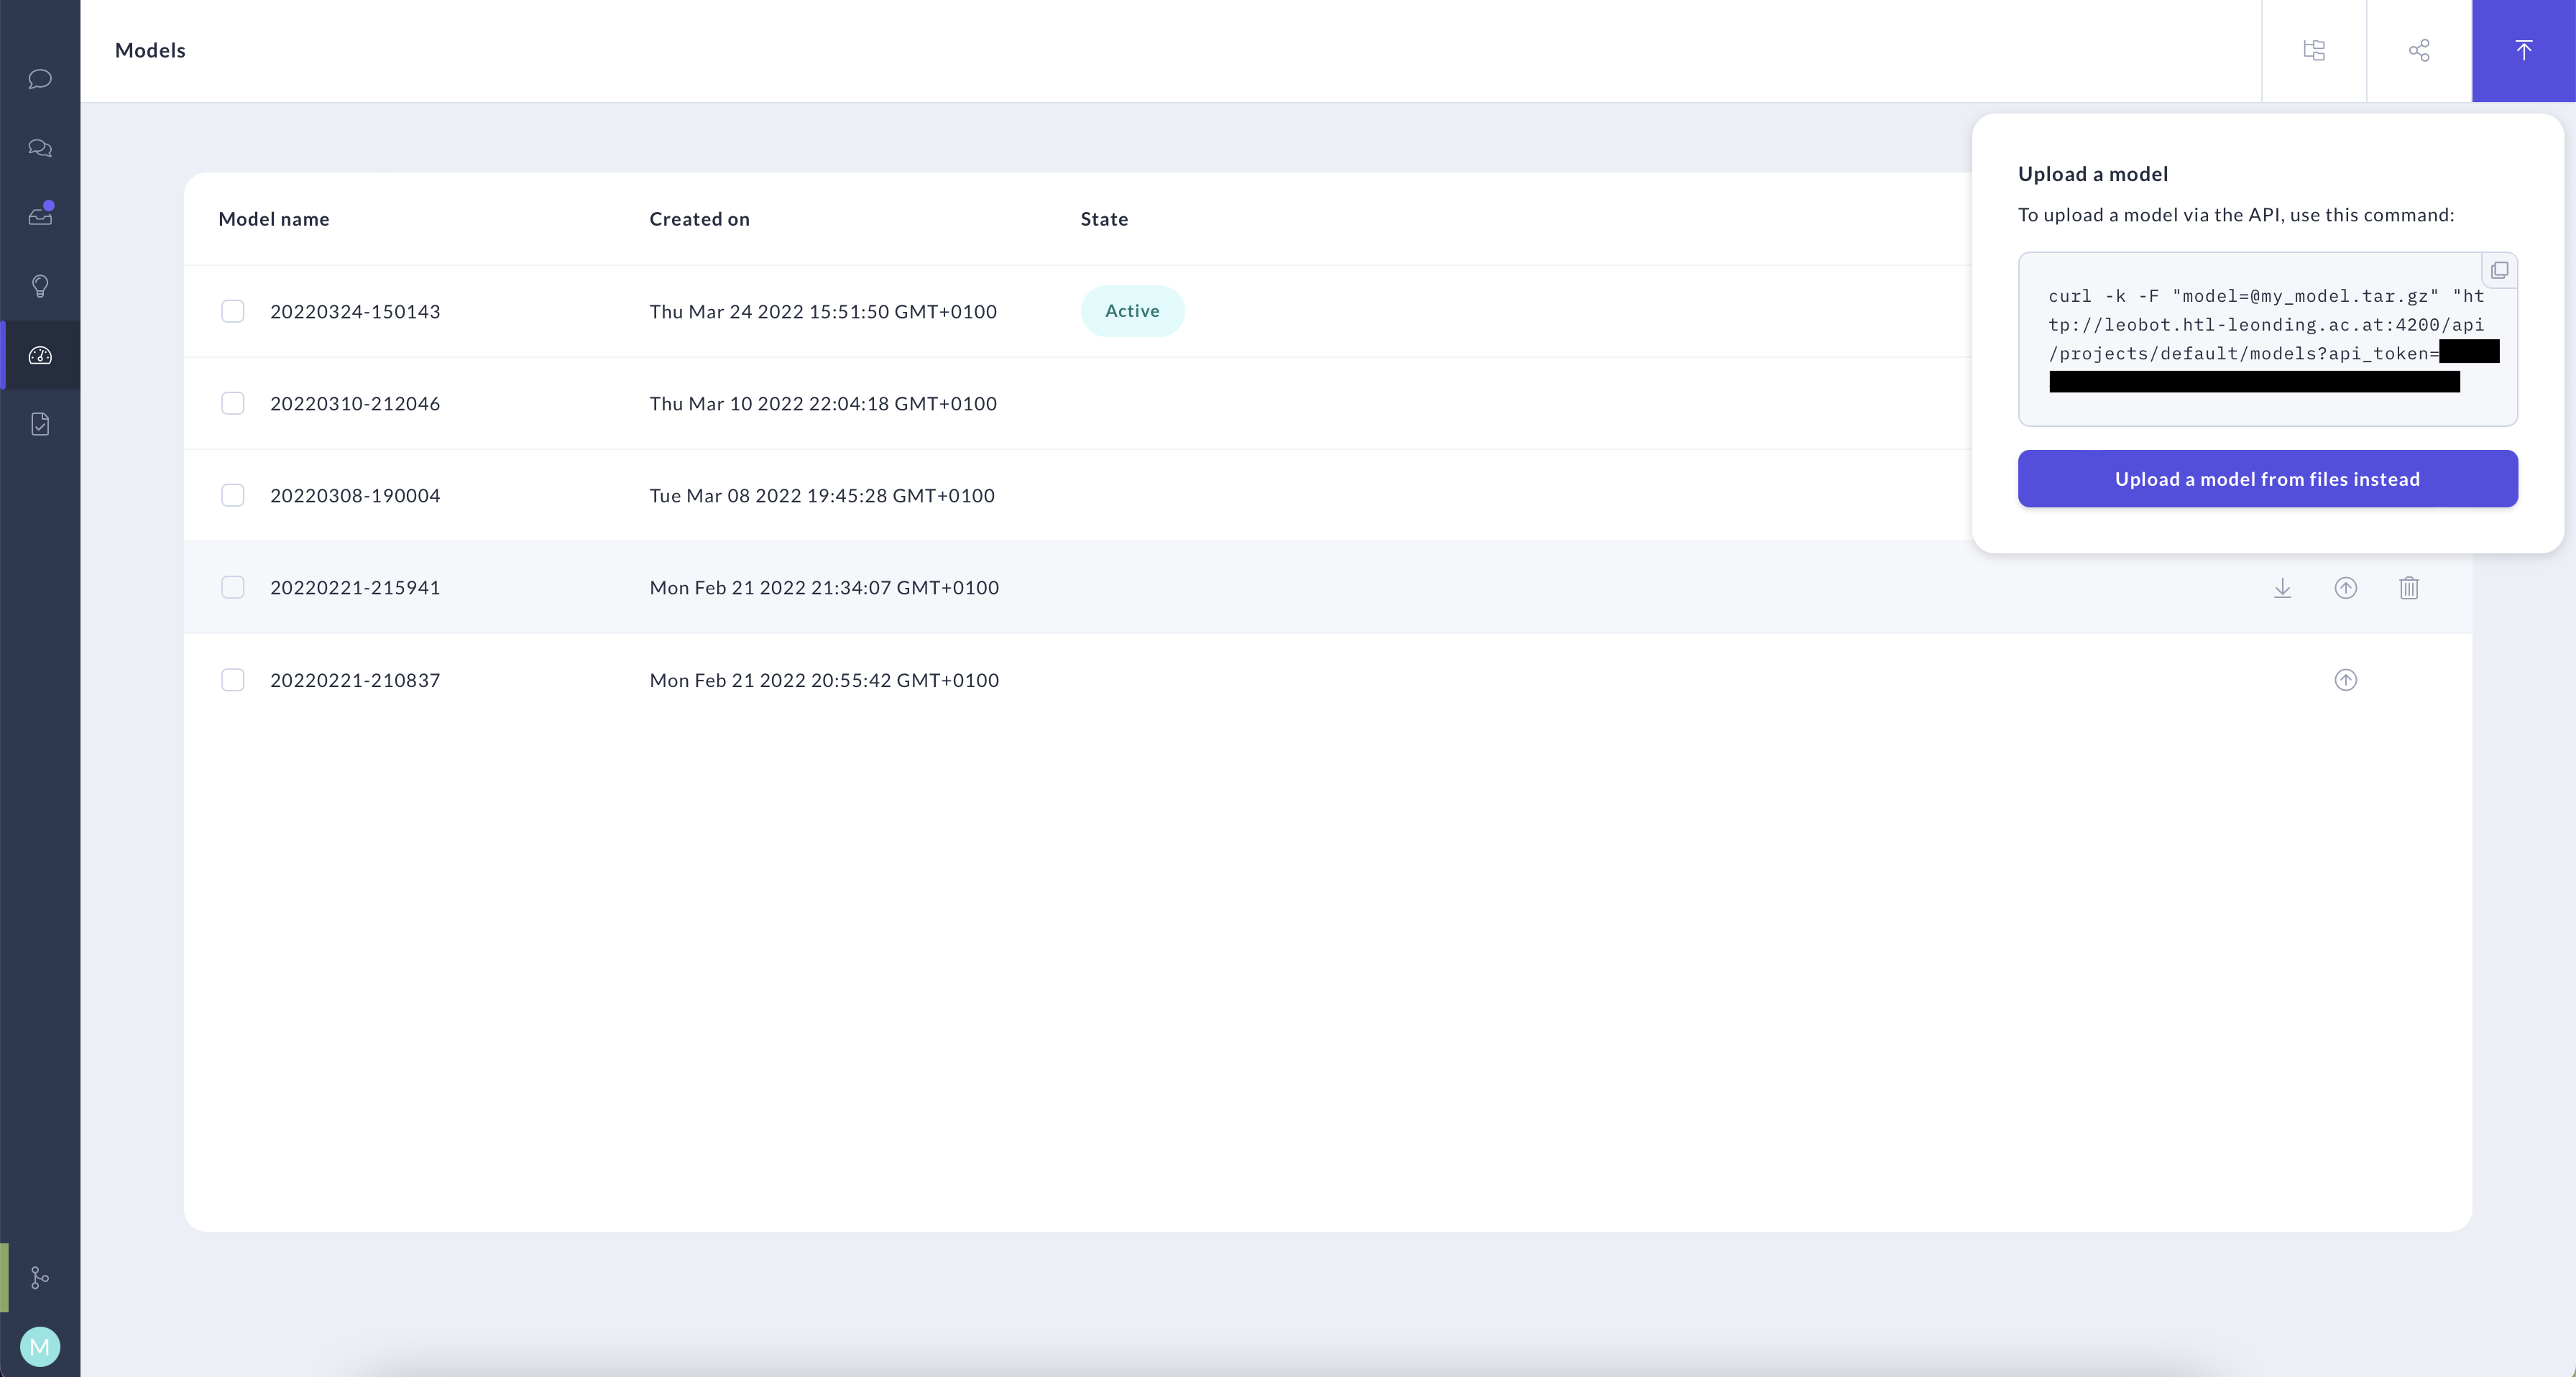
\includegraphics[scale=0.2]{pics/rasaxapimodel}
    \caption{Rasa X Oberfläche mit dem Befehl zum Model upload}
    \label{fig:impl:rasaxapimodel}
\end{figure}

\begin{lstlisting}[language=bash,label={lst:uploadlatestmodelshdefault},caption={Befehl zum Model Upload von Rasa X }]{Rasa X API Model Upload}
curl -k -F "model=@my_model.tar.gz" "http://leobot.htl-leonding.ac.at:4200/api/projects/default/models?api_token=TOKEN"
\end{lstlisting}

Dieser Befehl wurde angepasst sodass er immer das neuste Model hochlädt:

\begin{lstlisting}[language=bash,label={lst:uploadlatestmodelsh},caption={upload-latest-model.sh}]{upload-latest-model.sh}]
curl -k -F "model=@$(ls -t *tar.gz | head -1)" "localhost:4200/api/projects/default/models?api_token=TOKEN"
\end{lstlisting}

